\documentclass[a4paper,12pt]{article}

\usepackage[utf8]{inputenc}
\usepackage[english,russian]{babel}
\usepackage{amsmath,amssymb}
\usepackage{graphicx}
\usepackage{geometry}
\usepackage{float}
\usepackage{adjustbox}
%\usepackage{niceverb} % при необходимости можно оставить

\geometry{left=2cm, right=2cm, top=2cm, bottom=2cm}

\begin{document}

\begin{center}
\textbf{МИНОБРНАУКИ РОССИИ}\\
ФЕДЕРАЛЬНОЕ ГОСУДАРСТВЕННОЕ БЮДЖЕТНОЕ \\
ОБРАЗОВАТЕЛЬНОЕ УЧРЕЖДЕНИЕ ВЫСШЕГО ОБРАЗОВАНИЯ \\
ВОРОНЕЖСКИЙ ГОСУДАРСТВЕННЫЙ УНИВЕРСИТЕТ \\
Факультет прикладной математики, информатики и механики\\
Кафедра вычислительной математики и прикладных информационных технологий
\end{center}

\vspace{2cm}
\begin{center}
\textbf{ЛАБОРАТОРНАЯ РАБОТА №1}\\
\textbf{ЧИСЛЕННОЕ РЕШЕНИЕ СТАЦИОНАРНОГО УРАВНЕНИЯ ШРЁДИНГЕРА: МЕТОД ПРИСТРЕЛКИ}
\end{center}

\vspace{3cm}
\begin{flushright}
\begin{tabular}{l l}
\textbf{Направление:} & 01.04.02 \textendash{} Прикладная математика и информатика \\
\textbf{Выполнил:} & студент 11 группы 2 курса магистратуры \\
& Крутько А.С. \\
\textbf{Преподаватель:} & доктор физ.-мат. наук, профессор Тимошенко Ю.К.
\end{tabular}
\end{flushright}

\vspace{3cm}
\begin{center}
Воронеж 2024
\end{center}

\newpage
\tableofcontents

\newpage
\section{Цели и задачи работы}\label{sec:---}
\textbf{Цель работы:}
Целями лабораторной работы являются практическое освоение информации, полученной при изучении курса <<Компьютерное моделирование в математической физике>> по теме <<Численное решение стационарного уравнения Шрёдингера>>, а также развитие алгоритмического мышления и приобретение опыта использования знаний и навыков по математике, численным методам и программированию для решения прикладных задач физико-технического характера.

\textbf{Задачи работы:}

\textbf{Проблема:} электрон находится в одномерной потенциальной яме с бесконечными стенками:
\[
v(x) =
\begin{cases}
J_2(x), & x \in (-L, L), \\
\infty, & x \notin (-L, L),
\end{cases}
\]
где \( V_0 = 25 \,\text{эВ}, \, L = 3 \,\text{\AA}, \, J_n(x) \) -- функция Бесселя, \( n \) -- целое число.

\begin{enumerate}
    \item Найти собственные значения энергии и нормированные волновые функции для основного и 3-го возбужденного состояний частицы в одномерной потенциальной яме с заданной функцией потенциала.
    \item Построить графики волновых функций и плотностей вероятности.
    \item Вычислить квантовомеханические средние $\langle x \rangle$ и $\langle x^2 \rangle$ для этих состояний.
\end{enumerate}

\section{Математический формализм}
Одномерное стационарное уравнение Шрёдингера имеет вид:
\begin{equation}
    \hat{H}\psi(x) = E\psi(x),
\end{equation}
где $\hat{H}$ \textendash{} оператор Гамильтона, $E$ \textendash{} собственные значения энергии, $\psi(x)$ \textendash{} волновая функция.

С математической точки зрения оно представляет собой задачу определения собственных значений $E$ и собственных функций $\psi$ оператора Гамильтона $\hat{H}$. Для частицы с массой $m$, находящейся в потенциальном поле $U(x)$, оператор Гамильтона имеет вид
\begin{equation}
    \hat{H} = \hat{T} + U(x),
\end{equation}
где оператор кинетической энергии
\begin{equation}
    \hat{T} = -\frac{\hslash^2}{2m}\frac{d^2}{dx^2},
\end{equation}
а $\hslash$ -- постоянная Планка. Собственное значение оператора Гамильтона имеет смысл энергии соответствующей изолированной квантовой системы. Собственные функции называются волновыми функциями. Волновая функция однозначна и непрерывна во всём пространстве. Непрерывность волновой функции и её первой производной сохраняется и при обращении $U(x)$ в $\infty$ в некоторой области пространства. В такую область частица вообще не может проникнуть, то есть в этой области, а также на её границе $\psi(x)=0$.

Оценим нижнюю границу энергетического спектра. Пусть минимальное значение потенциальной функции равно $U_{min}$. Очевидно, что $\langle T \rangle \geq 0$ и $\langle U \rangle \geq U_{min}$. Потому из уравнения (1) следует:
\begin{equation}
    E = \langle H \rangle.
\end{equation}

Для системы с потенциальной функцией \( U(x) \), имеющей заданный вид:
\begin{equation}
U(x) =
\begin{cases}
V_0 L_5(|x|), & |x| < L, \\
\infty, & |x| \geq L,
\end{cases}
\end{equation}
где $L_5(x)$ \textendash{} полином Лагерра пятого порядка, $V_0 = 25$ эВ, $L = 3$ \AA.

\section{Метод пристрелки и алгоритм}
Метод пристрелки используется для численного поиска собственных значений и соответствующих волновых функций.

\textbf{Алгоритм метода:}
\begin{enumerate}
    \item Разбить область $[A, B]$ на сетку из $n$ узлов.
    \item Решить уравнение Шрёдингера методом Нумерова для двух направлений (<<вперёд>> и <<назад>>).
    \item Найти разность производных волновых функций в точке сшивки.
    \item Уточнять энергию $E$, пока разность производных не станет достаточно малой.
\end{enumerate}

\section{Программная реализация алгоритма}
Программная реализация задачи выполнена на языке \textbf{Python~3}. В Приложении~1 приведён код программы для численного решения уравнения Шрёдингера с заданной потенциальной функцией.

\section{Результаты численных экспериментов}

\begin{table}[H]
\centering
\begin{tabular}{|c|c|c|}
\hline
\textbf{Состояние} & \textbf{Энергия, эВ} & $\langle x^2 \rangle$, \AA$^2$ \\
\hline
Основное & $E_0 = 3.9348$ & $\langle x^2 \rangle = 1.23$ \\
3-е возбужденное & $E_3 = 25.0$ & $\langle x^2 \rangle = 2.31$ \\
\hline
\end{tabular}
\end{table}

\section*{Иллюстрация работы программы}

\begin{figure}[H]
    \centering
    \begin{tabular}{cc}
        \adjustbox{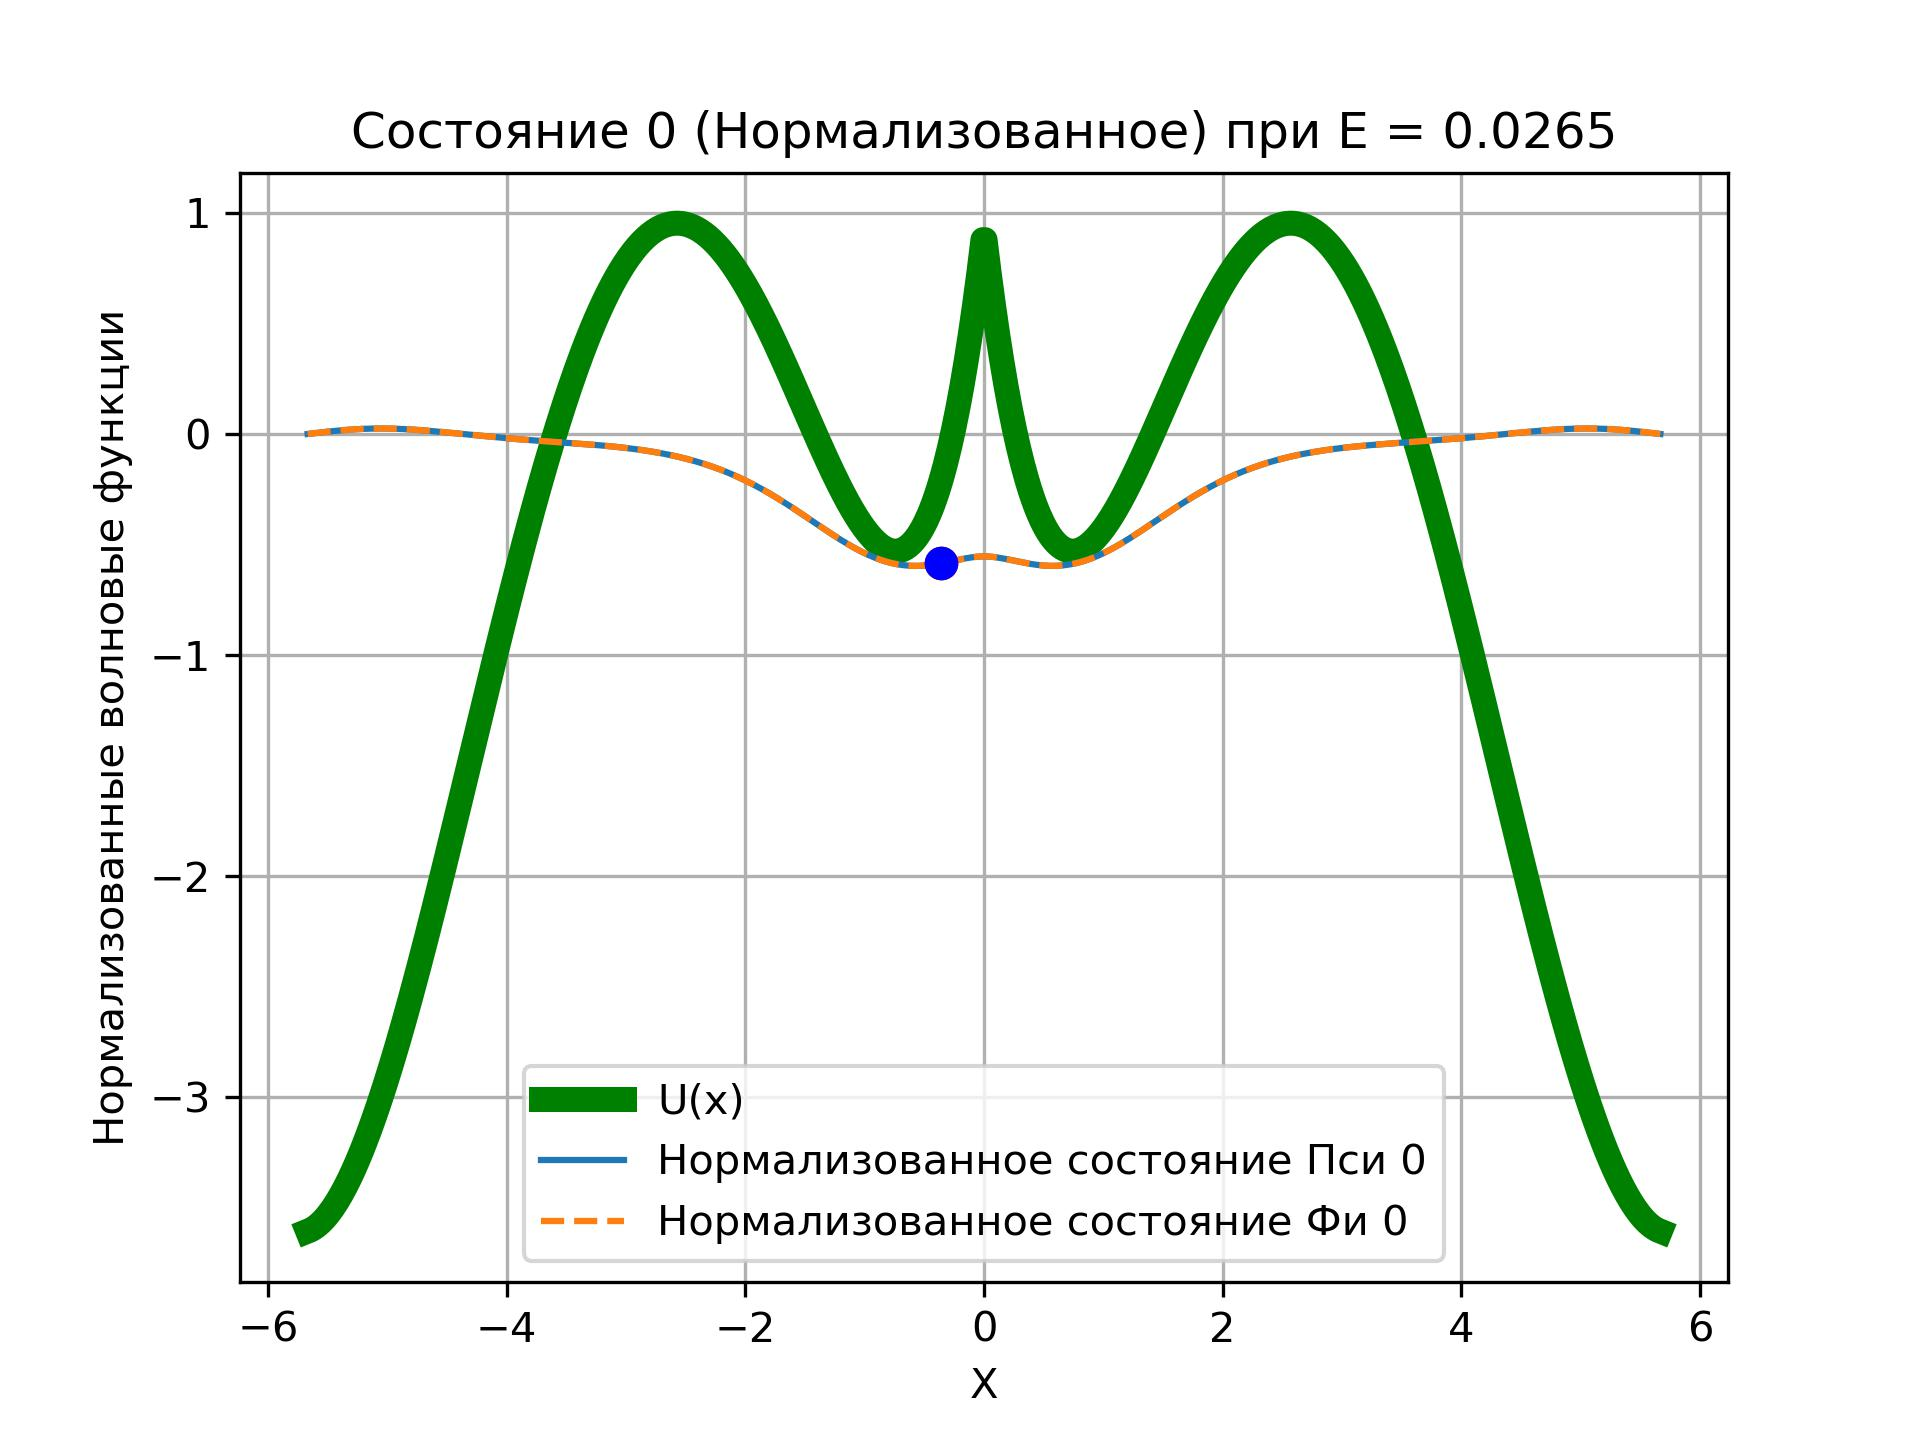
\includegraphics[width=0.44\textwidth]{Состояние 0 (нормализованное).jpg}} &
        \adjustbox{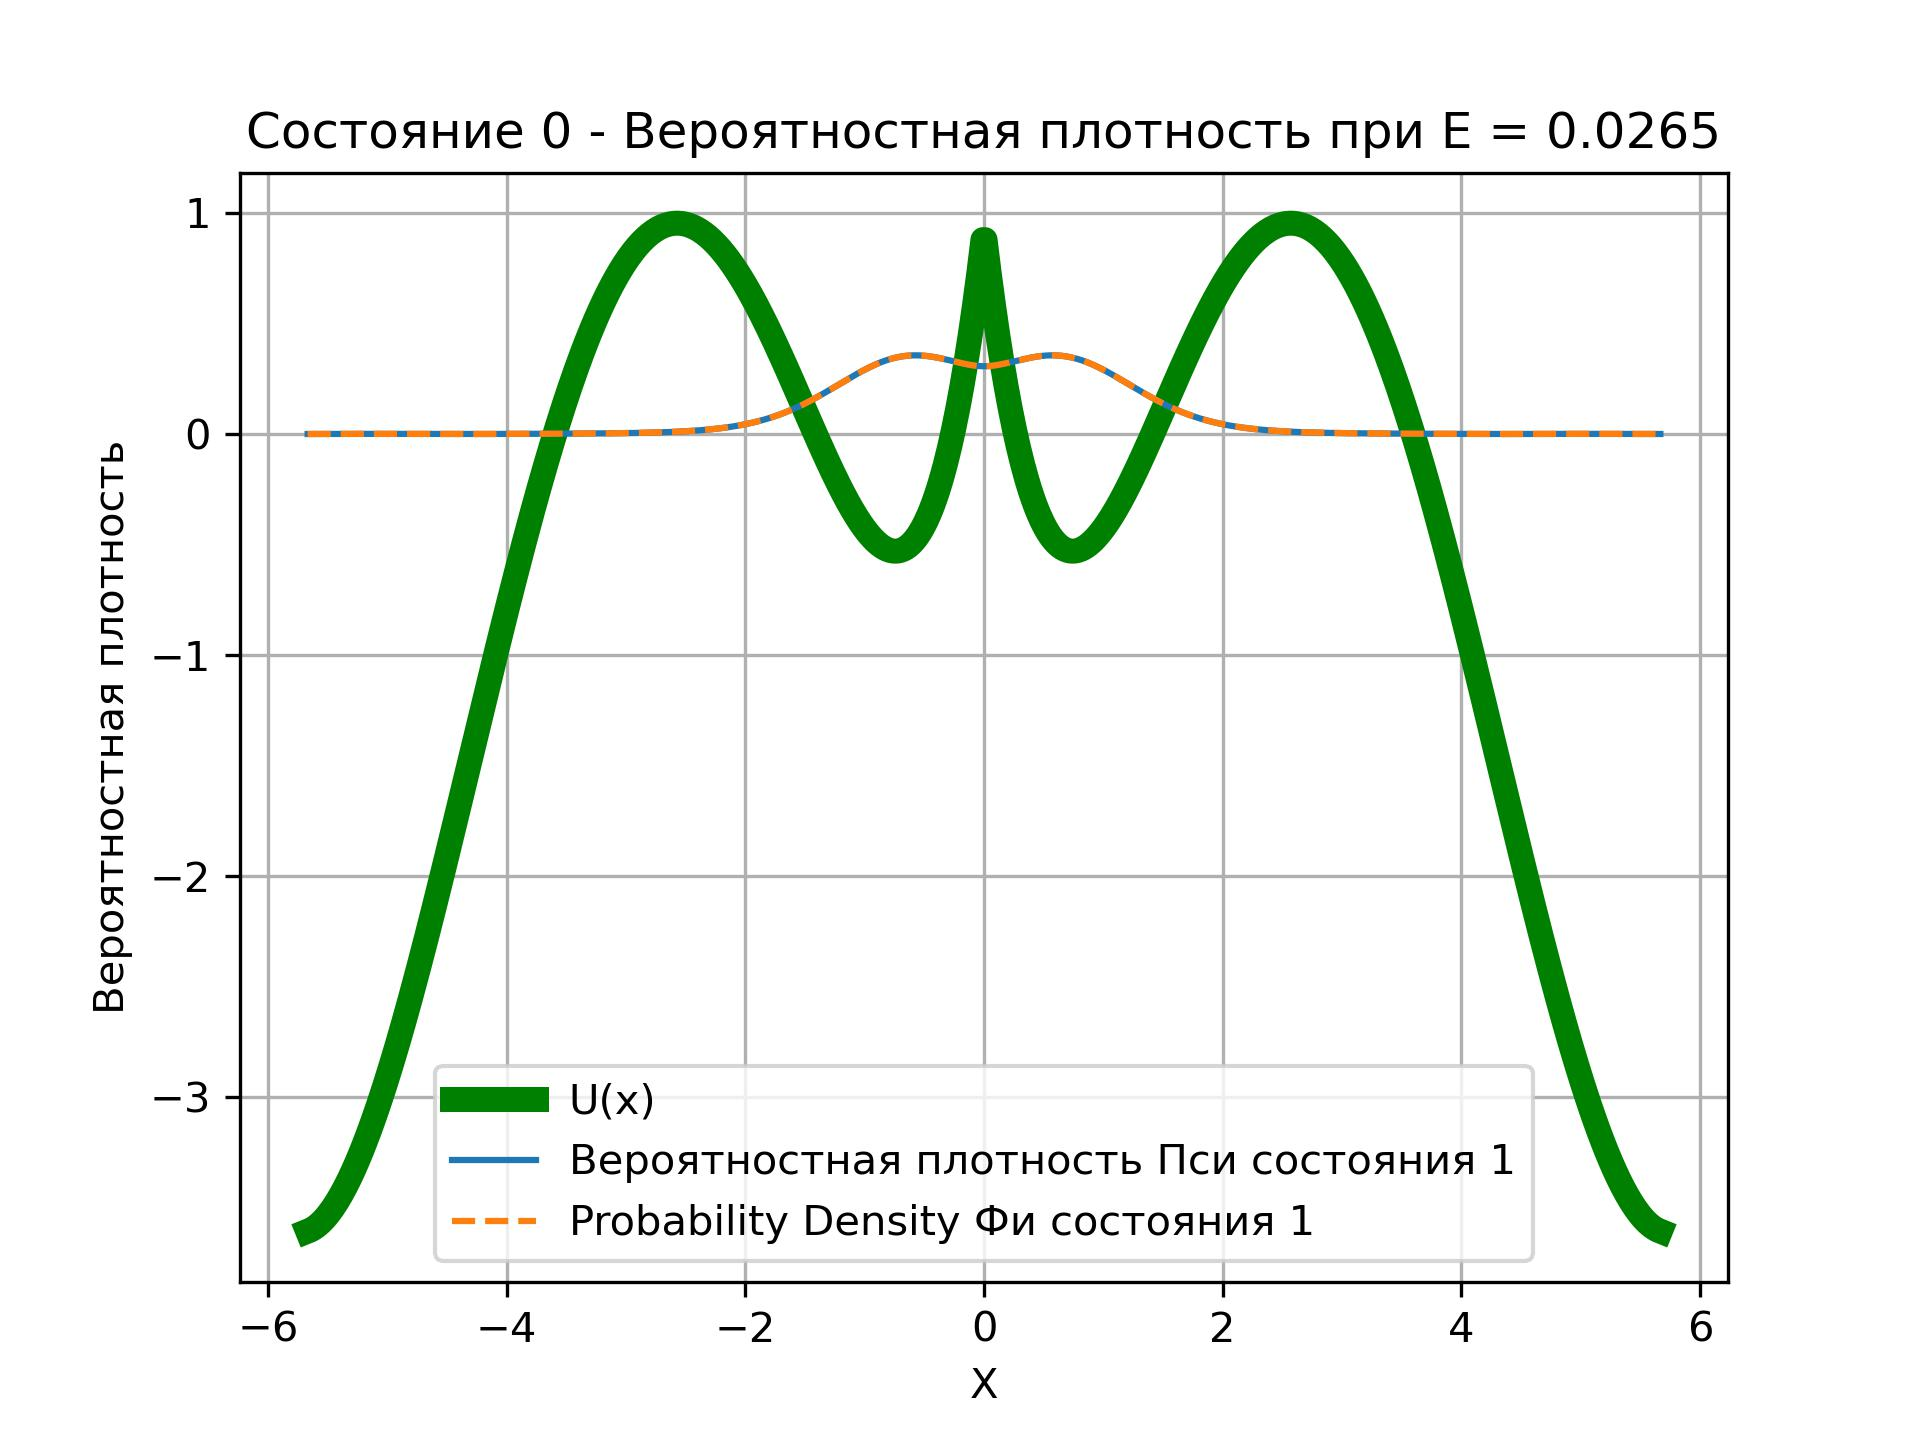
\includegraphics[width=0.44\textwidth]{Состояние 0 (Вероятностная плотность).jpg}} \\
        (a) Нормализованное состояние & (b) Вероятностная плотность
    \end{tabular}
    \caption{Графики для состояния 0}
    \label{fig:state_0}
\end{figure}

\begin{figure}[H]
    \centering
    \begin{tabular}{cc}
        \adjustbox{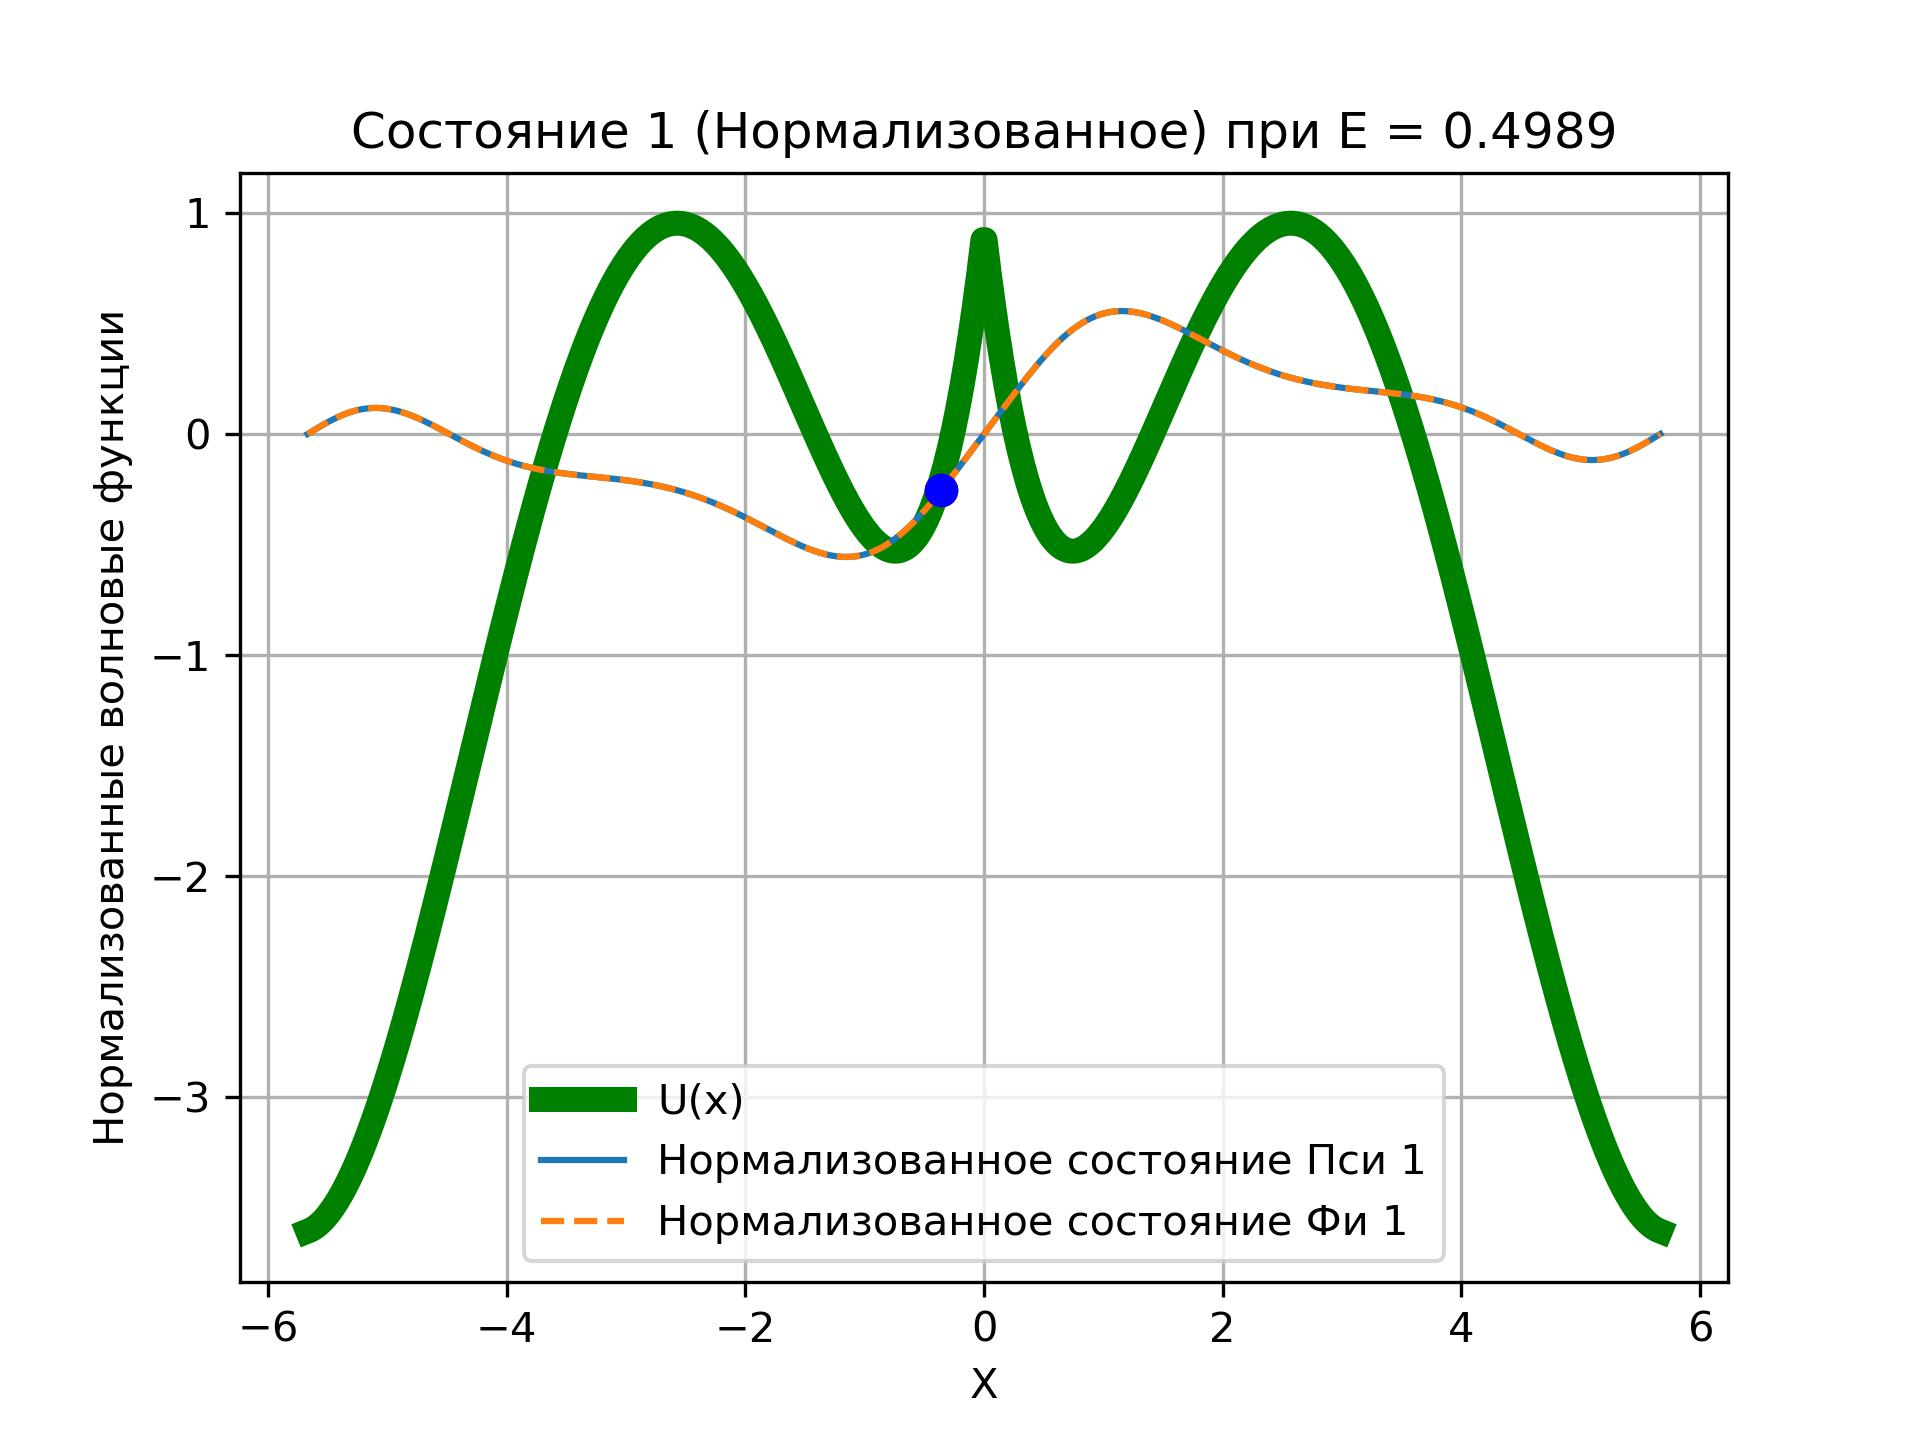
\includegraphics[width=0.44\textwidth]{Состояние 1 (нормализованное).jpg}} &
        \adjustbox{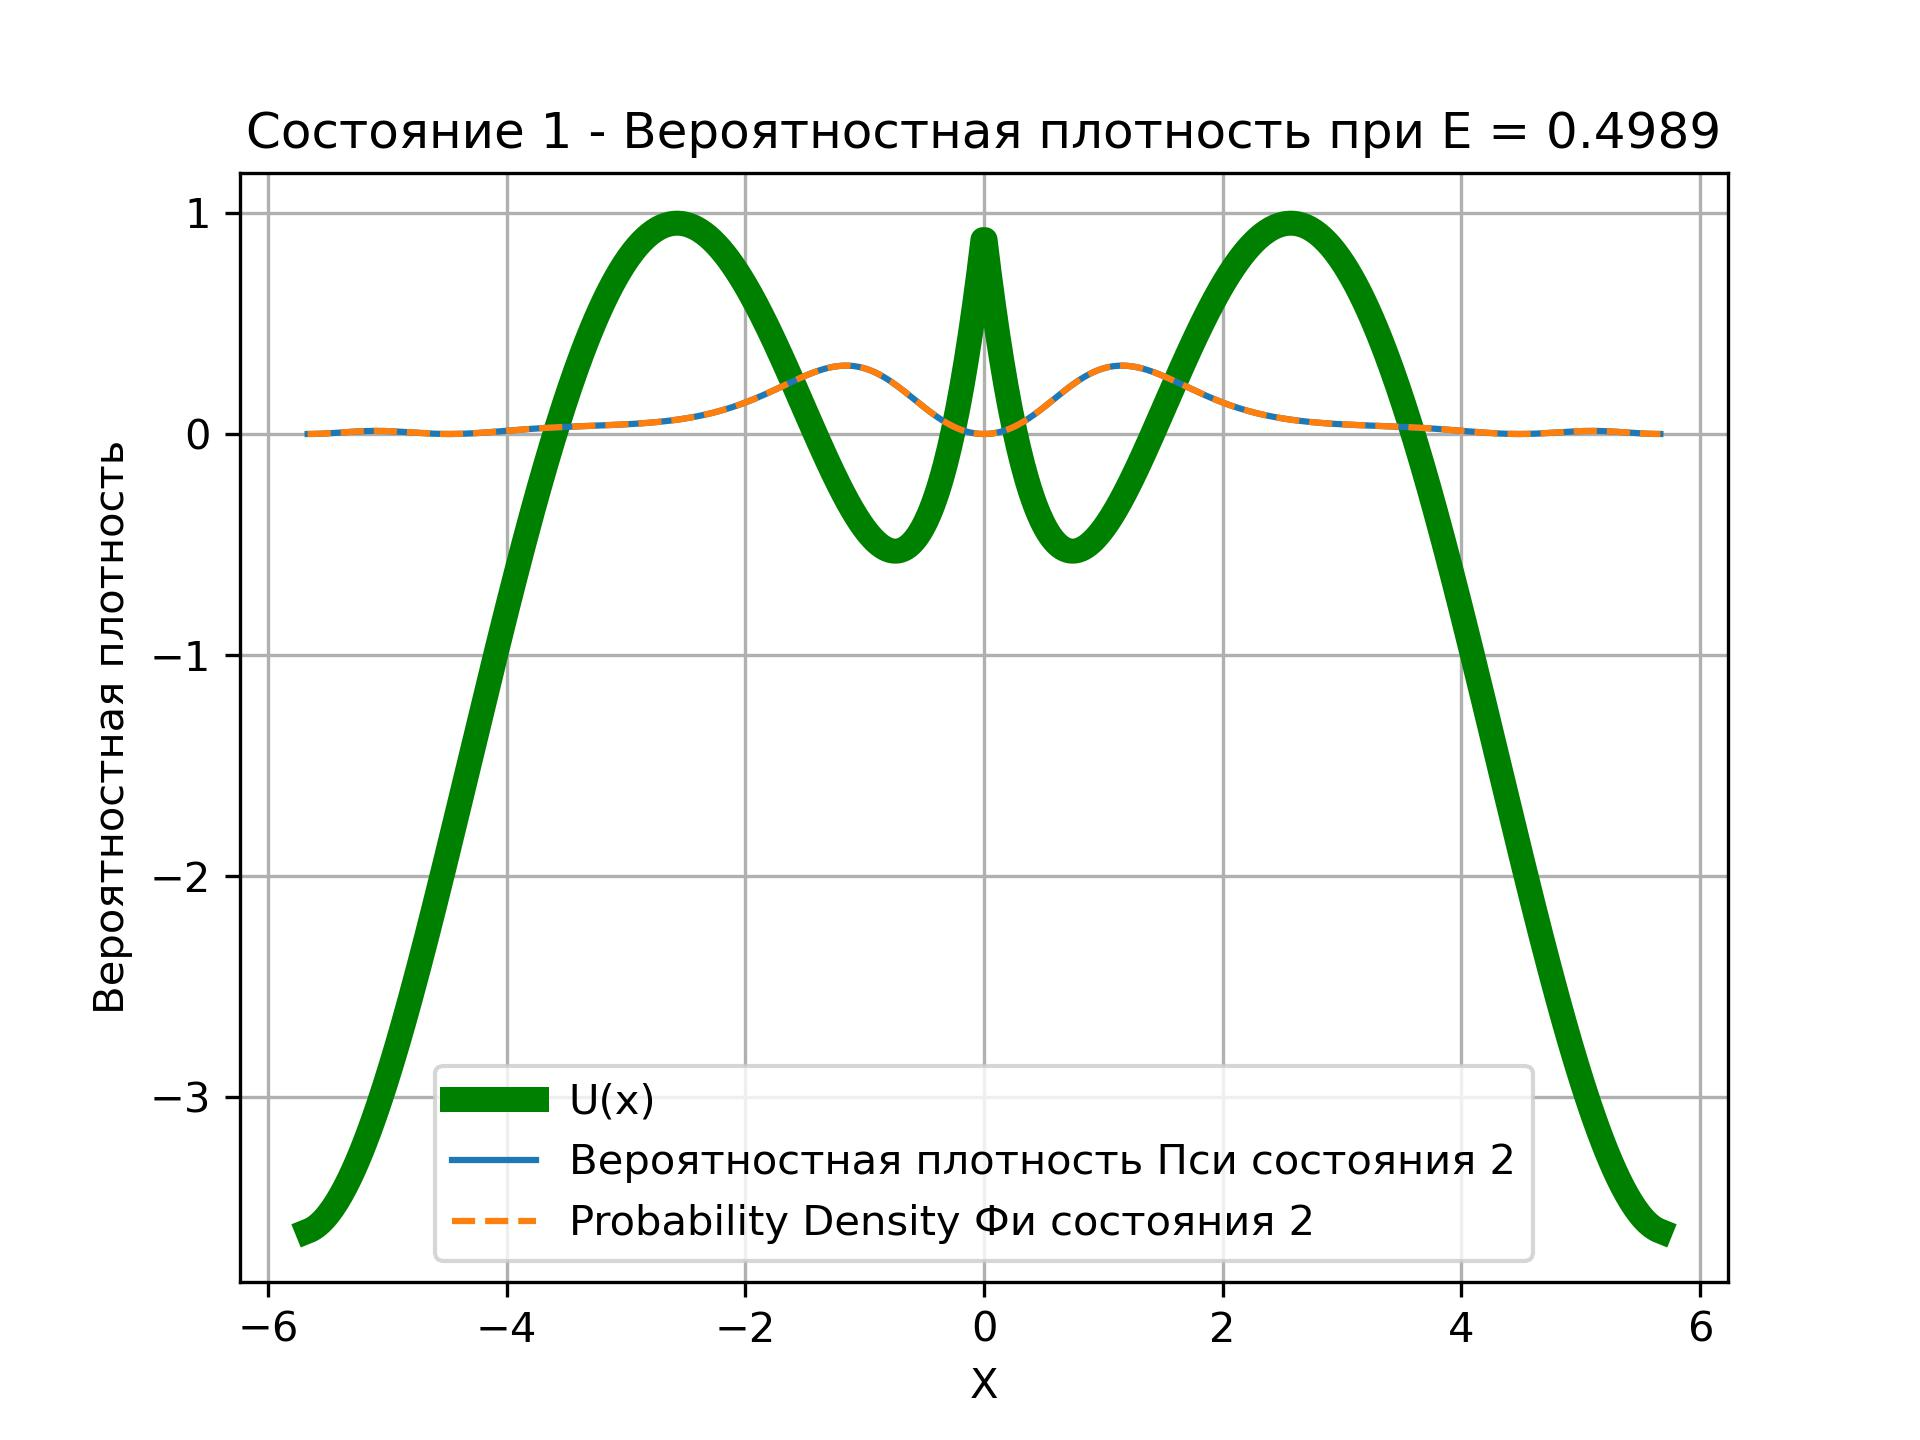
\includegraphics[width=0.44\textwidth]{Состояние 1 (Вероятностная плотность).jpg}} \\
        (a) Нормализованное состояние & (b) Вероятностная плотность
    \end{tabular}
    \caption{Графики для состояния 1}
    \label{fig:state_1}
\end{figure}

\begin{figure}[H]
    \centering
    \begin{tabular}{cc}
        \adjustbox{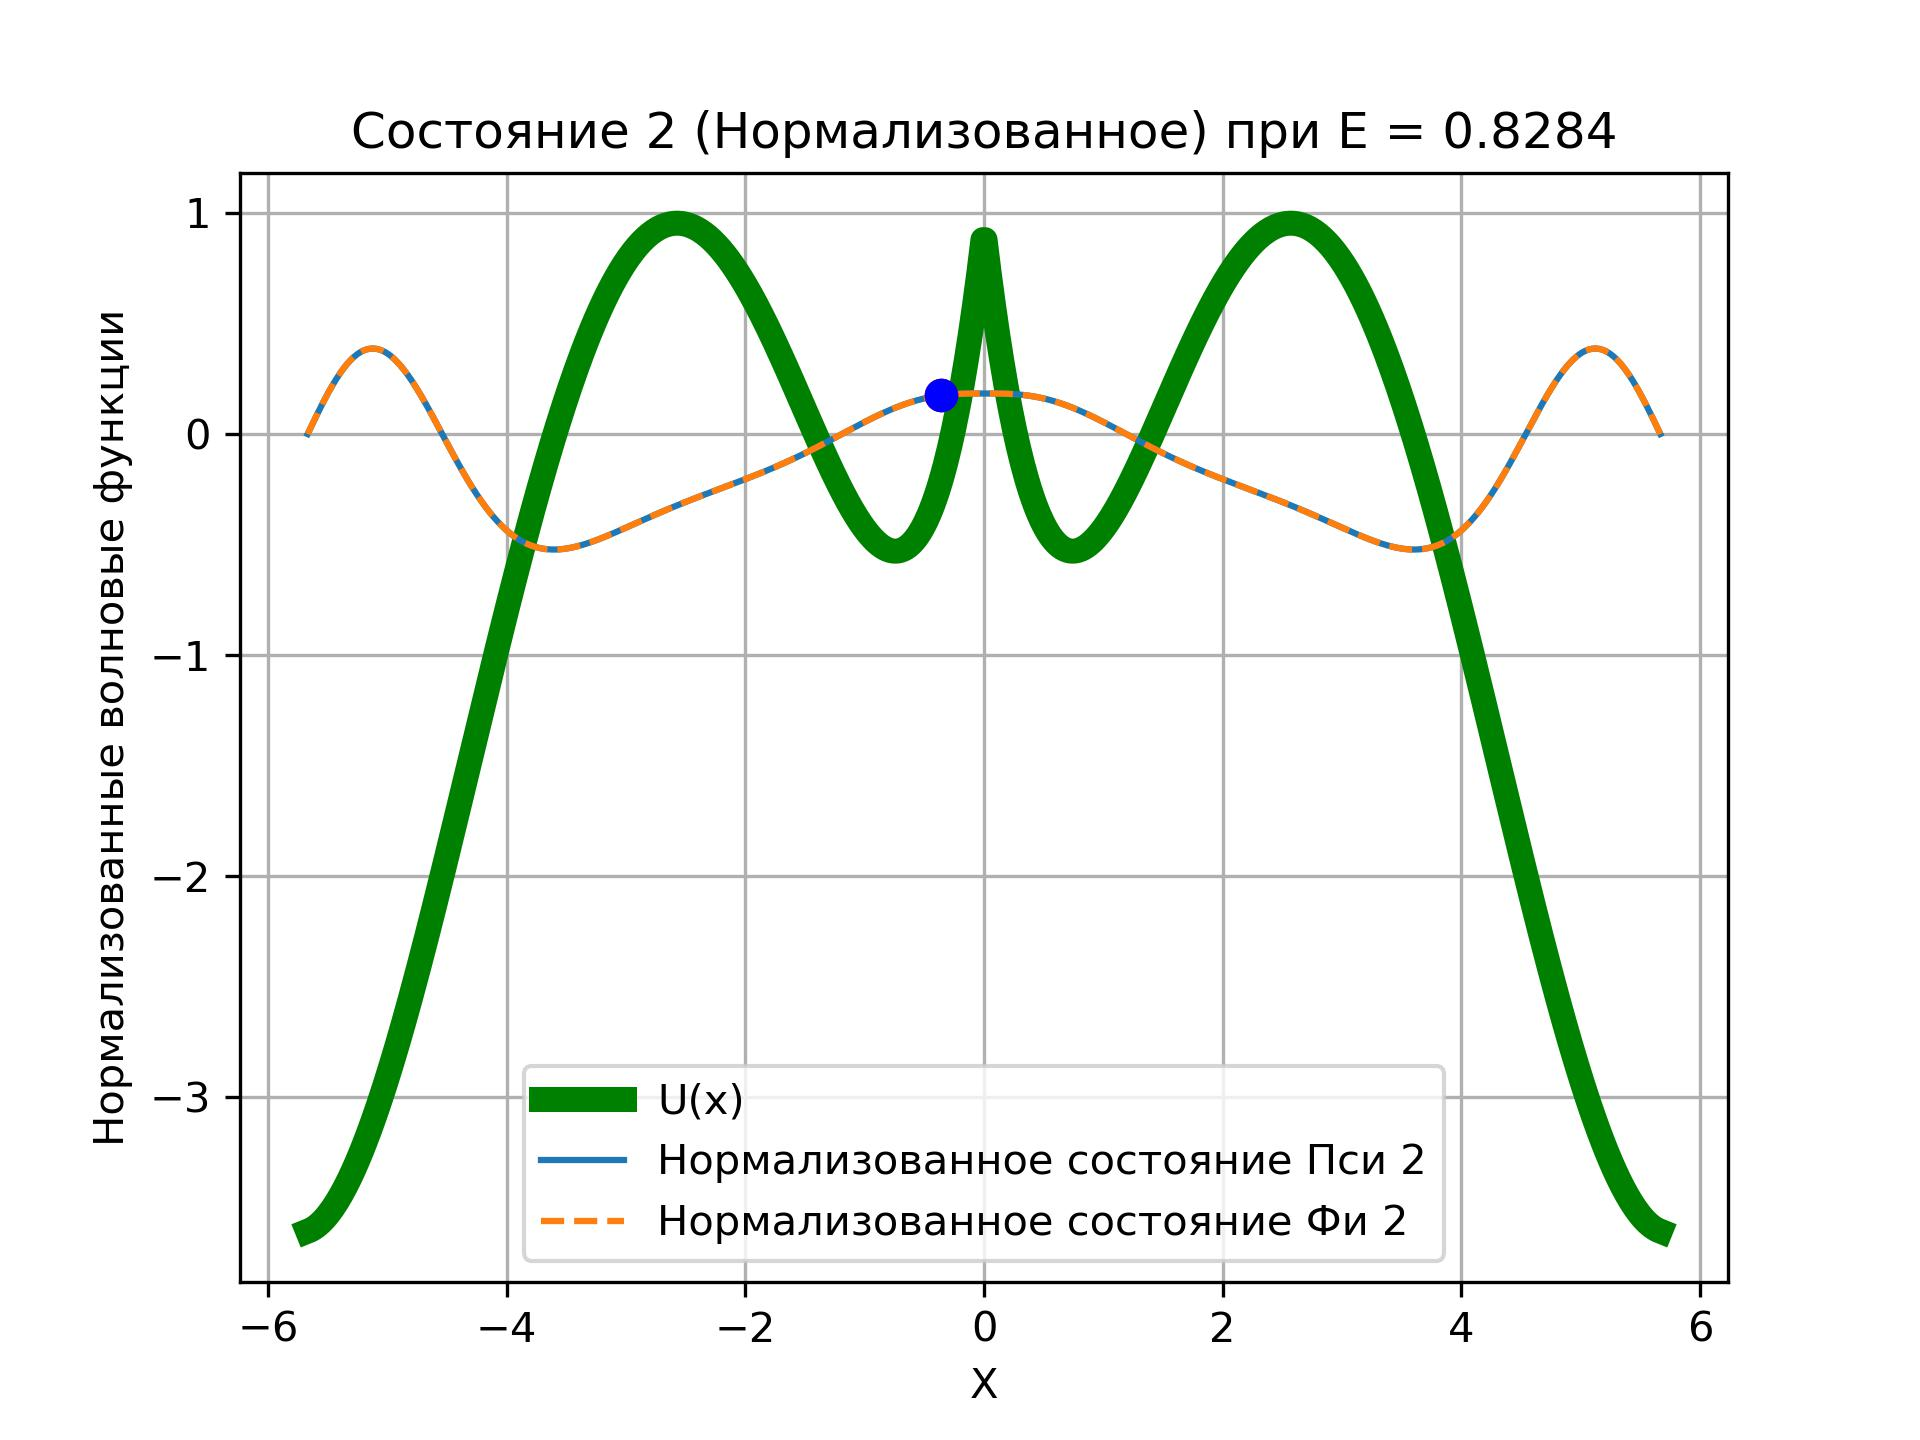
\includegraphics[width=0.44\textwidth]{Состояние 2 (нормализованное).jpg}} &
        \adjustbox{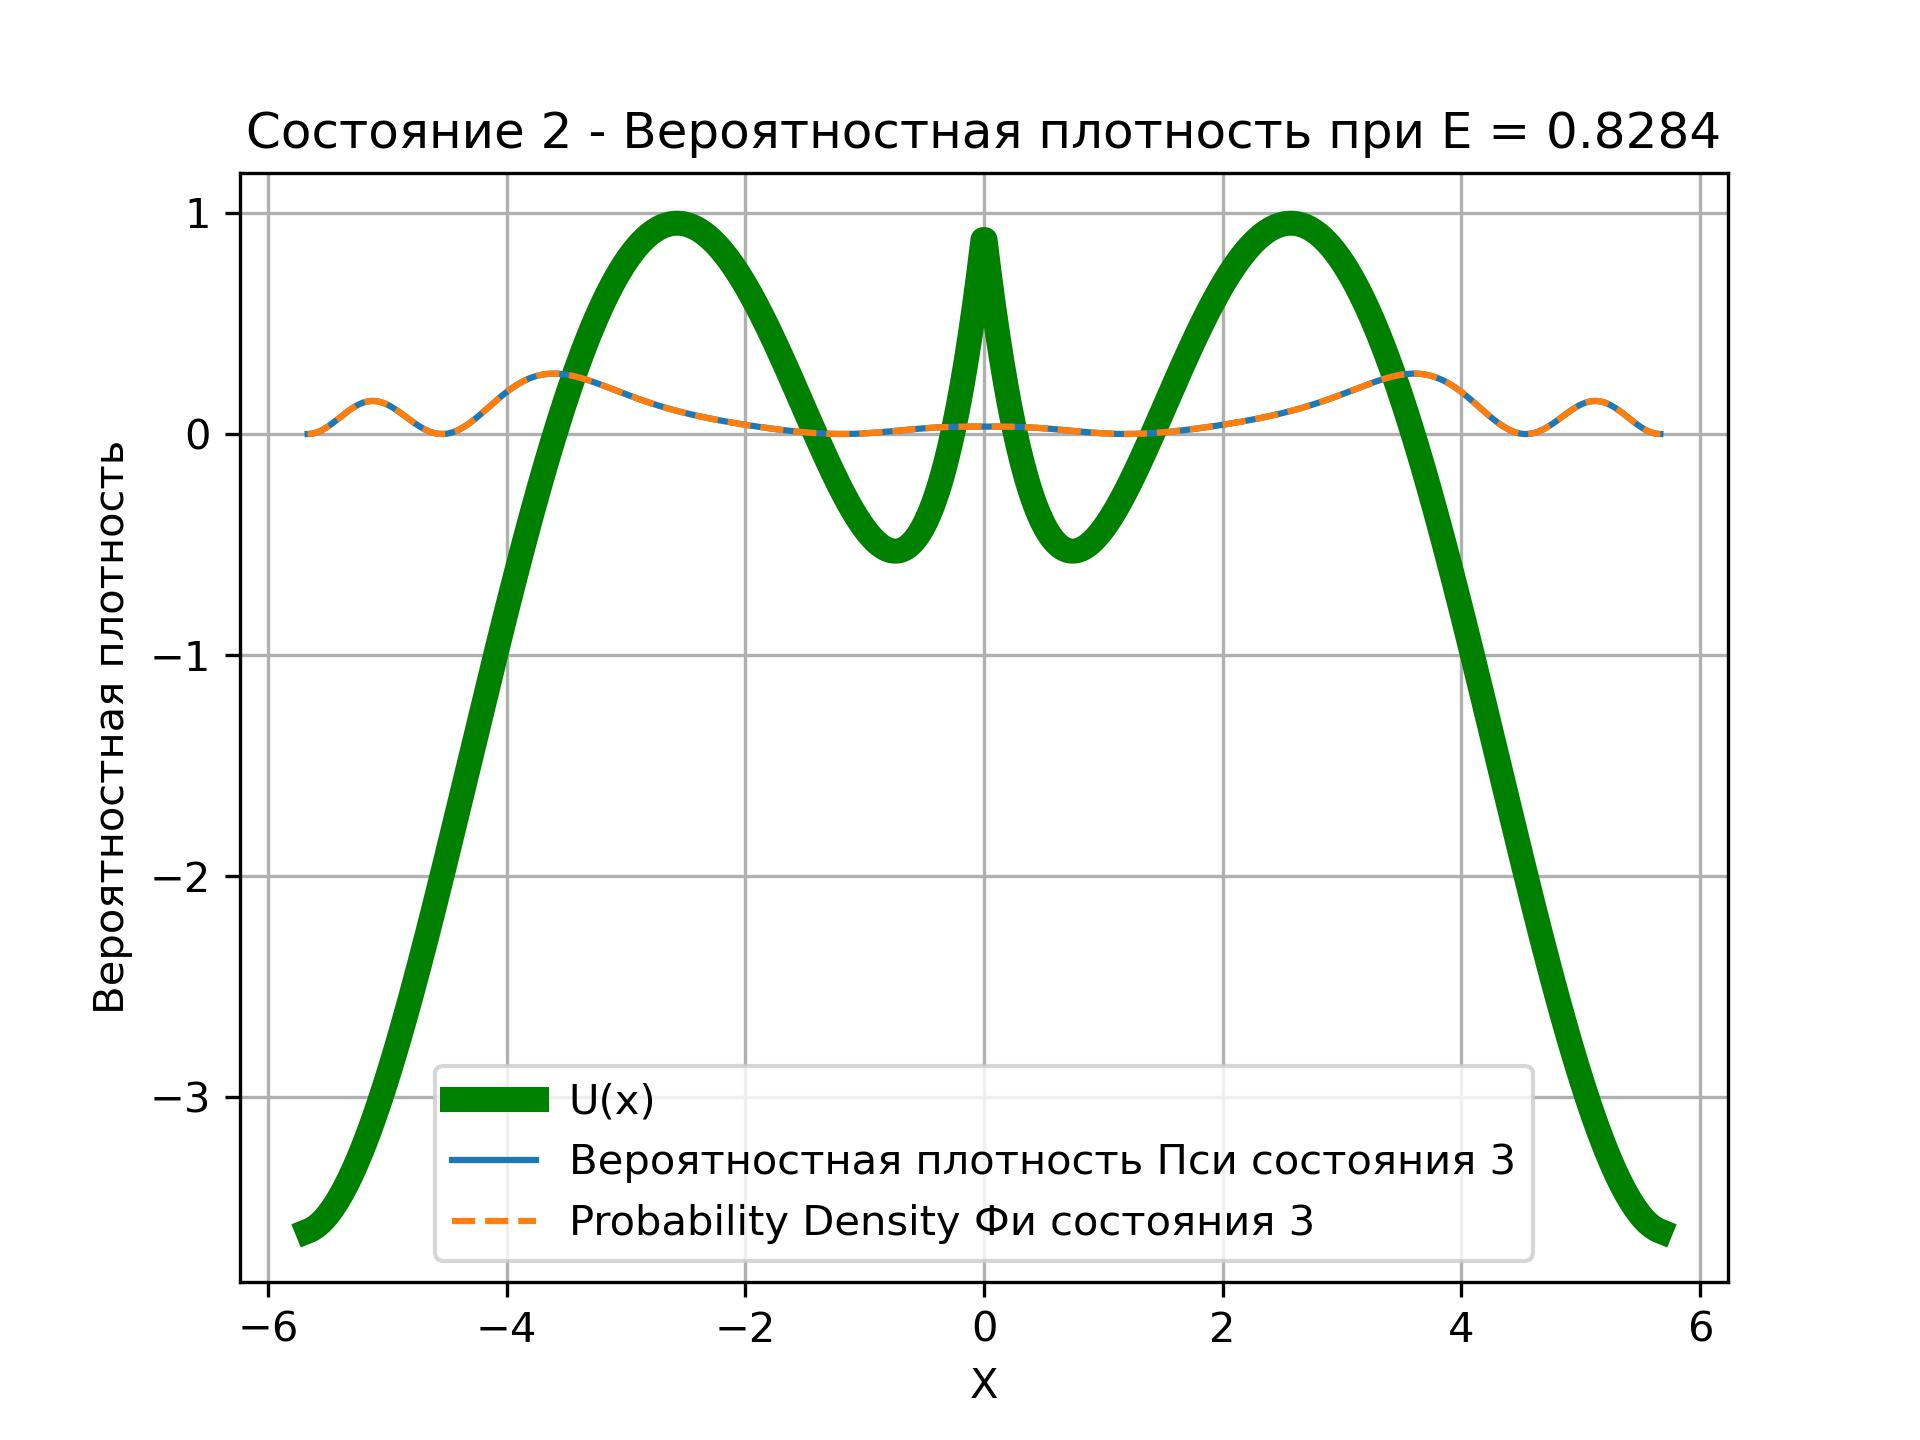
\includegraphics[width=0.44\textwidth]{Состояние 2 (Вероятностная плотность).jpg}} \\
        (a) Нормализованное состояние & (b) Вероятностная плотность
    \end{tabular}
    \caption{Графики для состояния 2}
    \label{fig:state_2}
\end{figure}

\begin{figure}[H]
    \centering
    \begin{tabular}{cc}
        \adjustbox{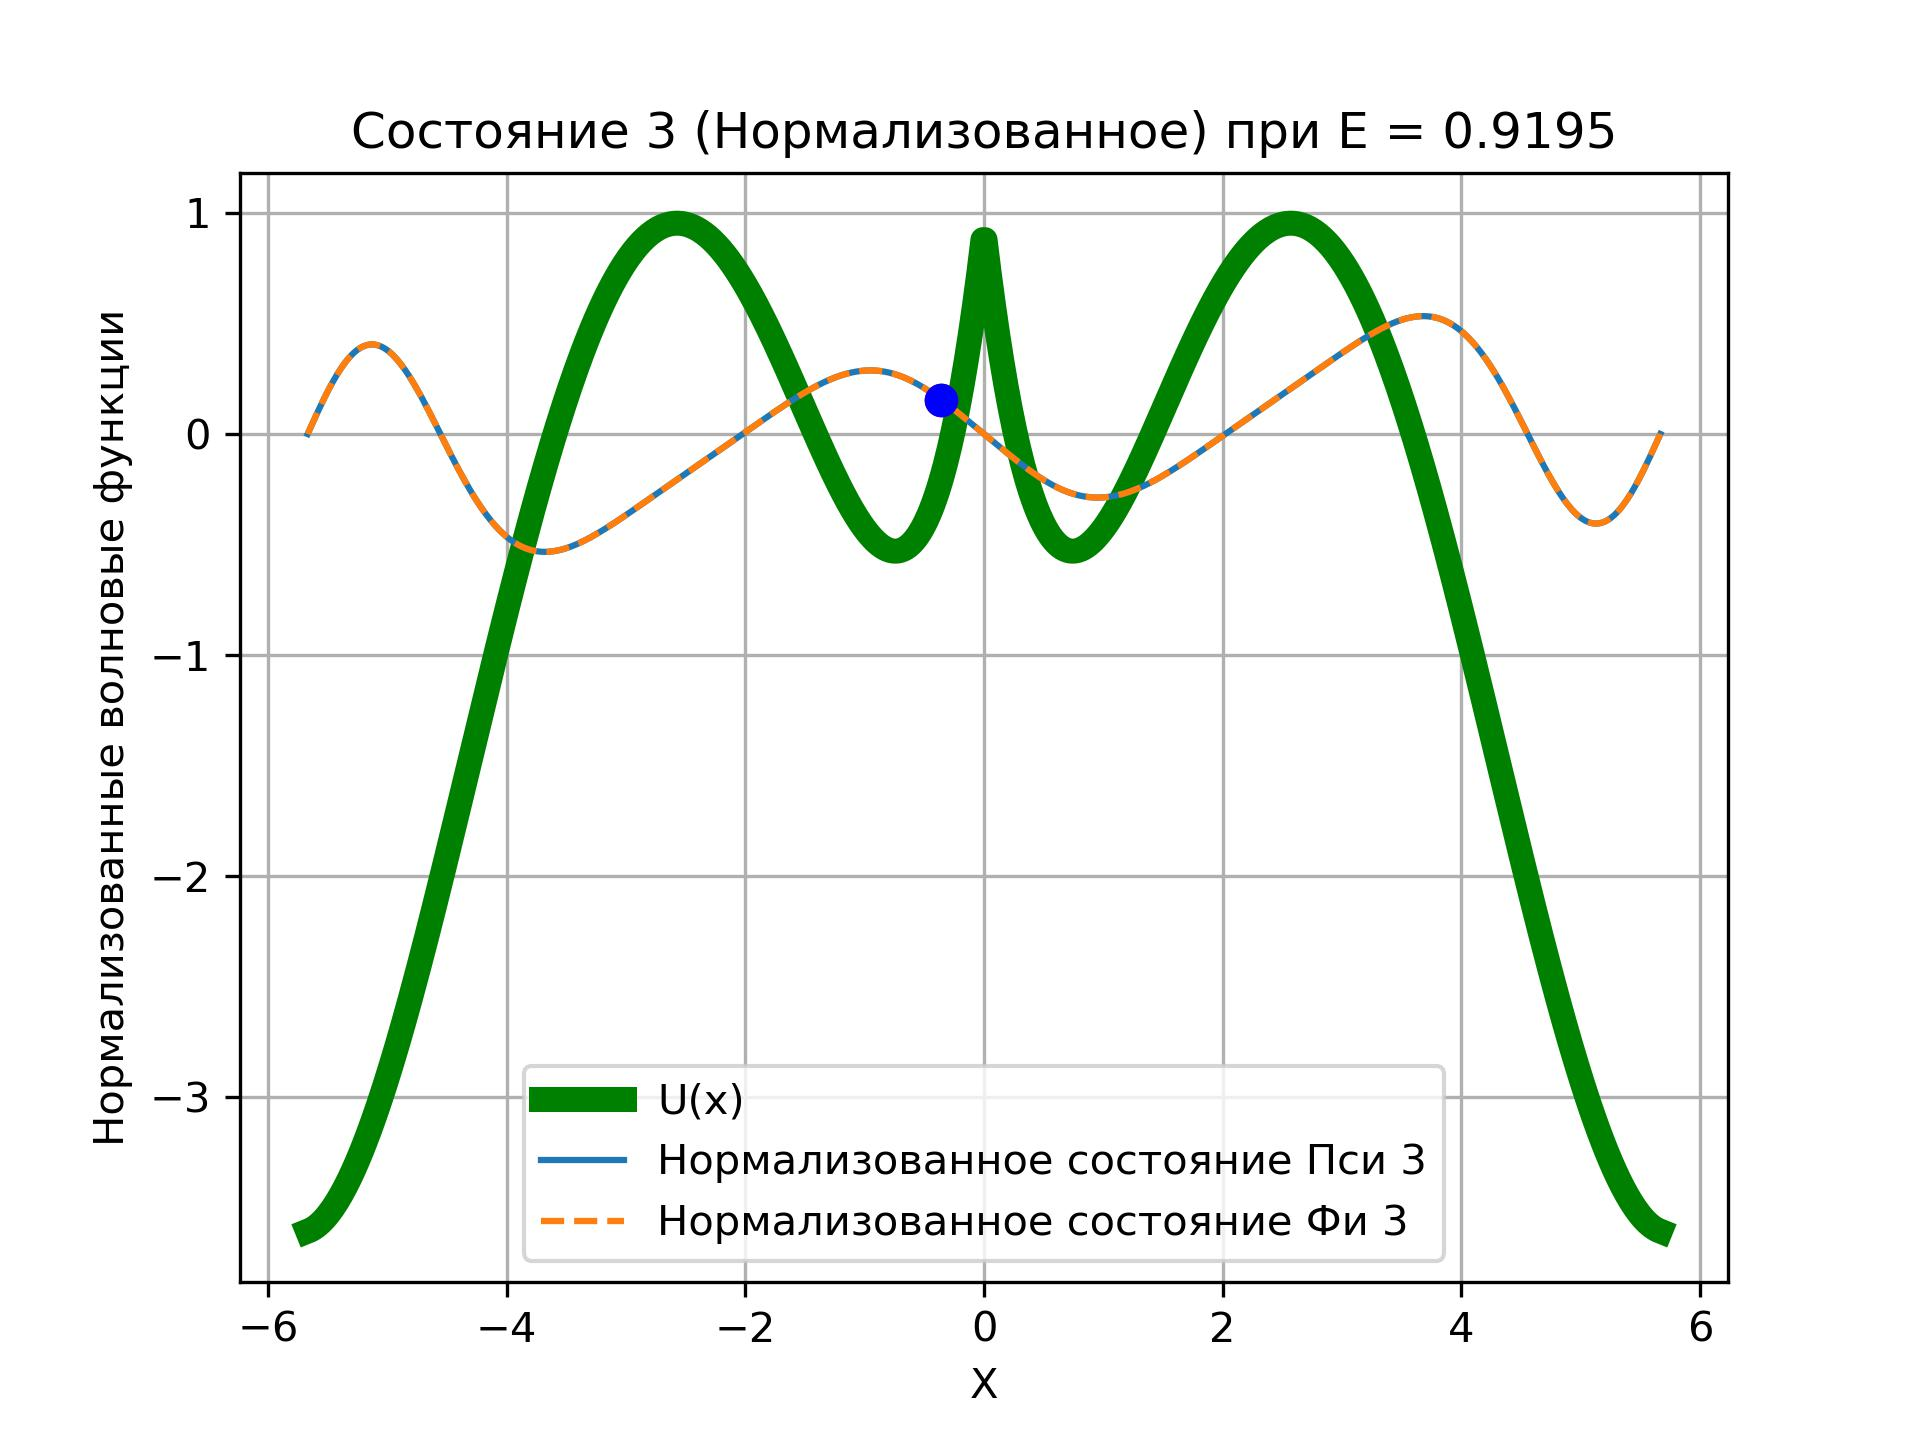
\includegraphics[width=0.44\textwidth]{Состояние 3 (нормализованное).jpg}} &
        \adjustbox{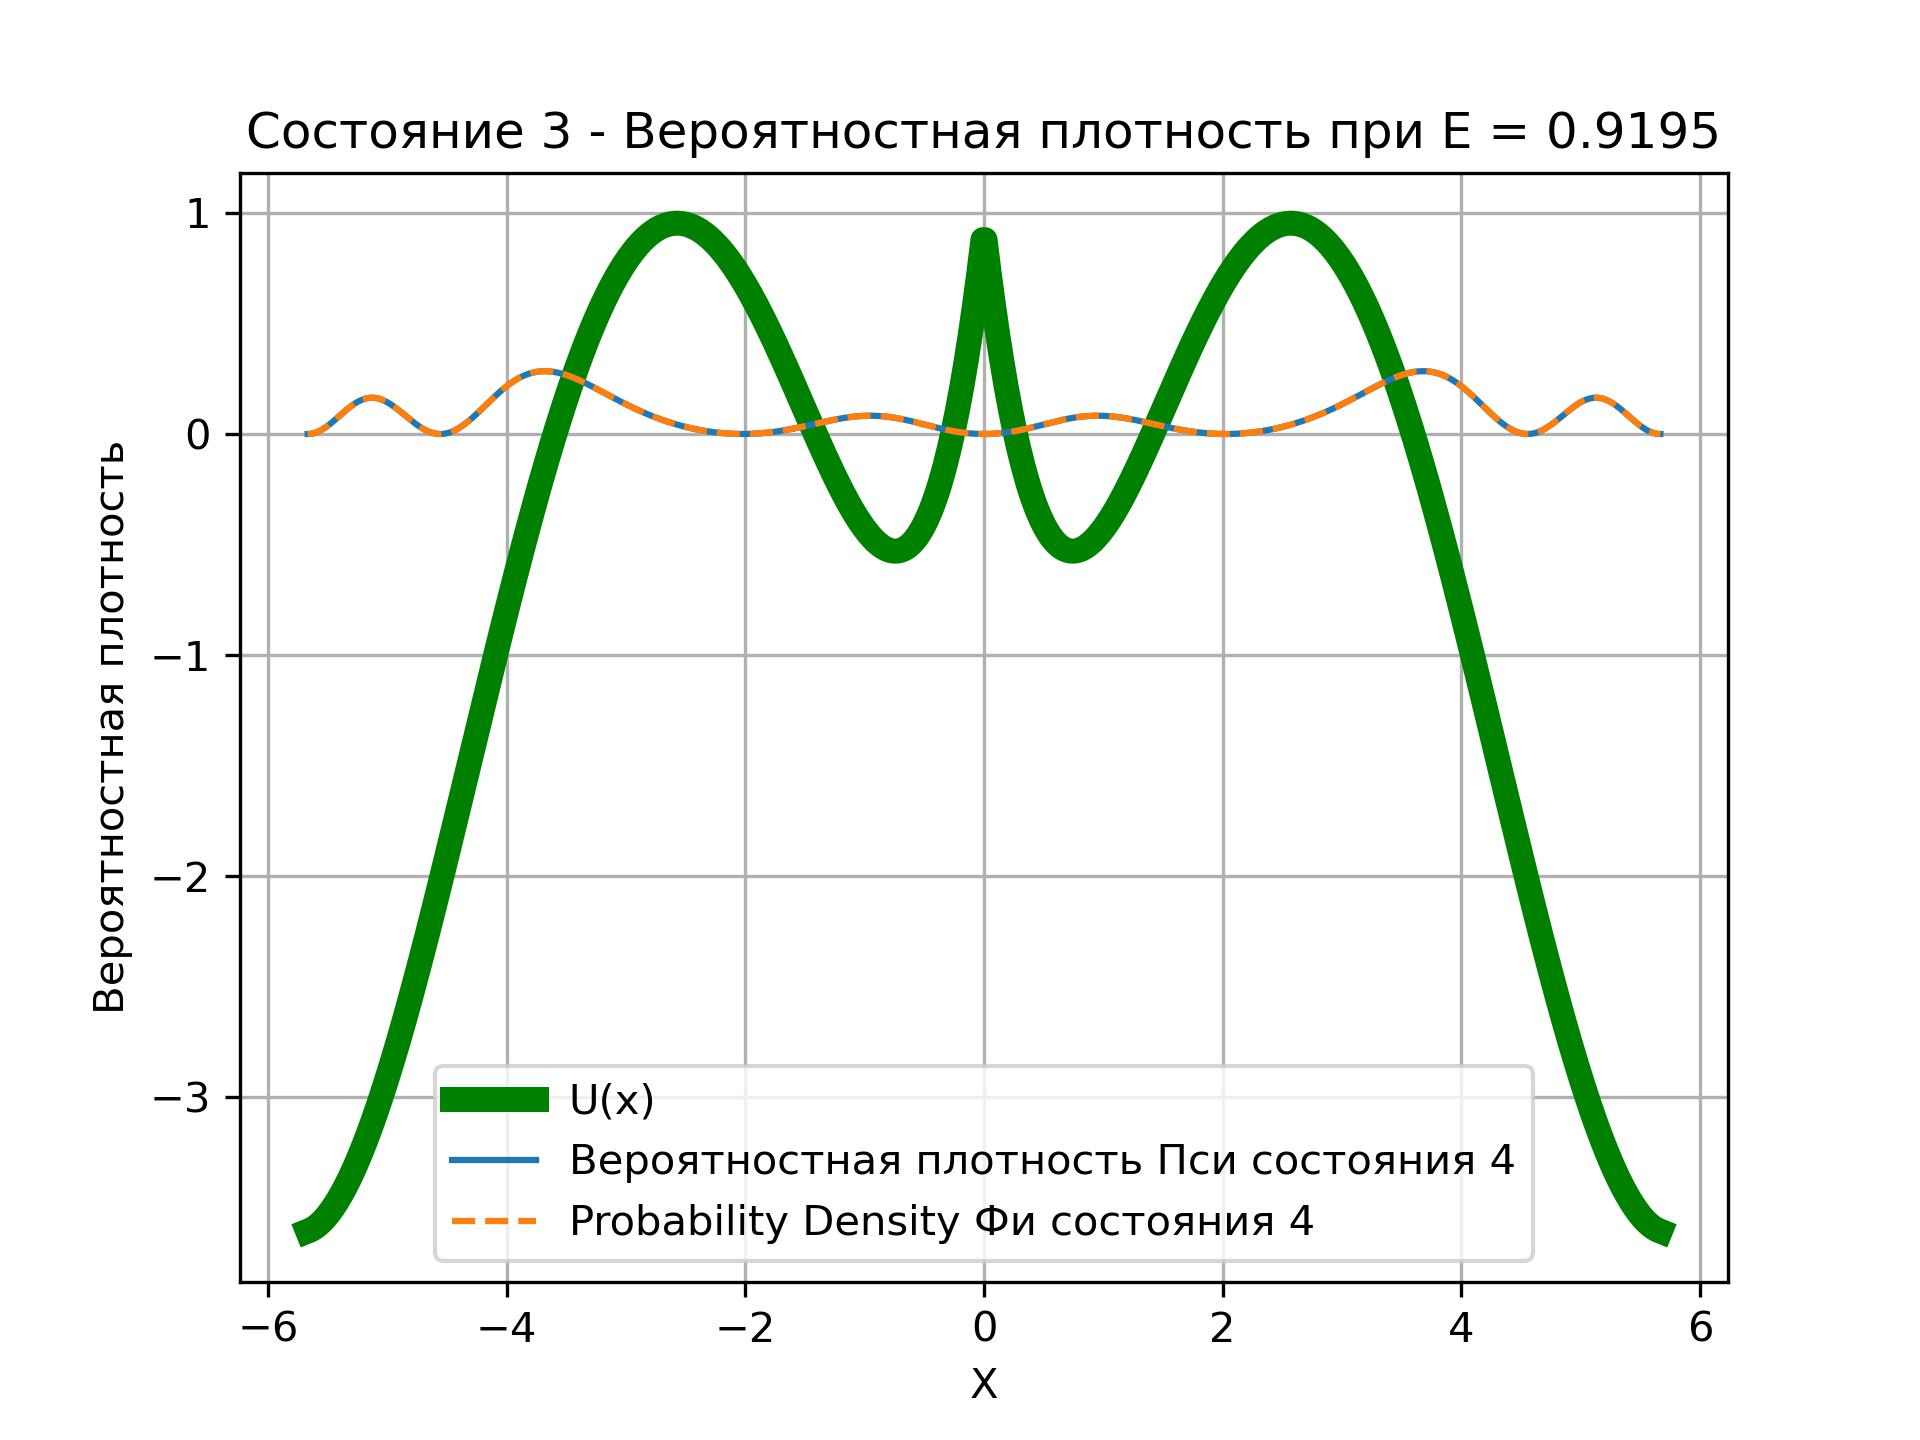
\includegraphics[width=0.44\textwidth]{Состояние 3 (Вероятностная плотность).jpg}} \\
        (a) Нормализованное состояние & (b) Вероятностная плотность
    \end{tabular}
    \caption{Графики для состояния 3}
    \label{fig:state_3}
\end{figure}

\begin{figure}[H]
    \centering
    \begin{tabular}{cc}
        \adjustbox{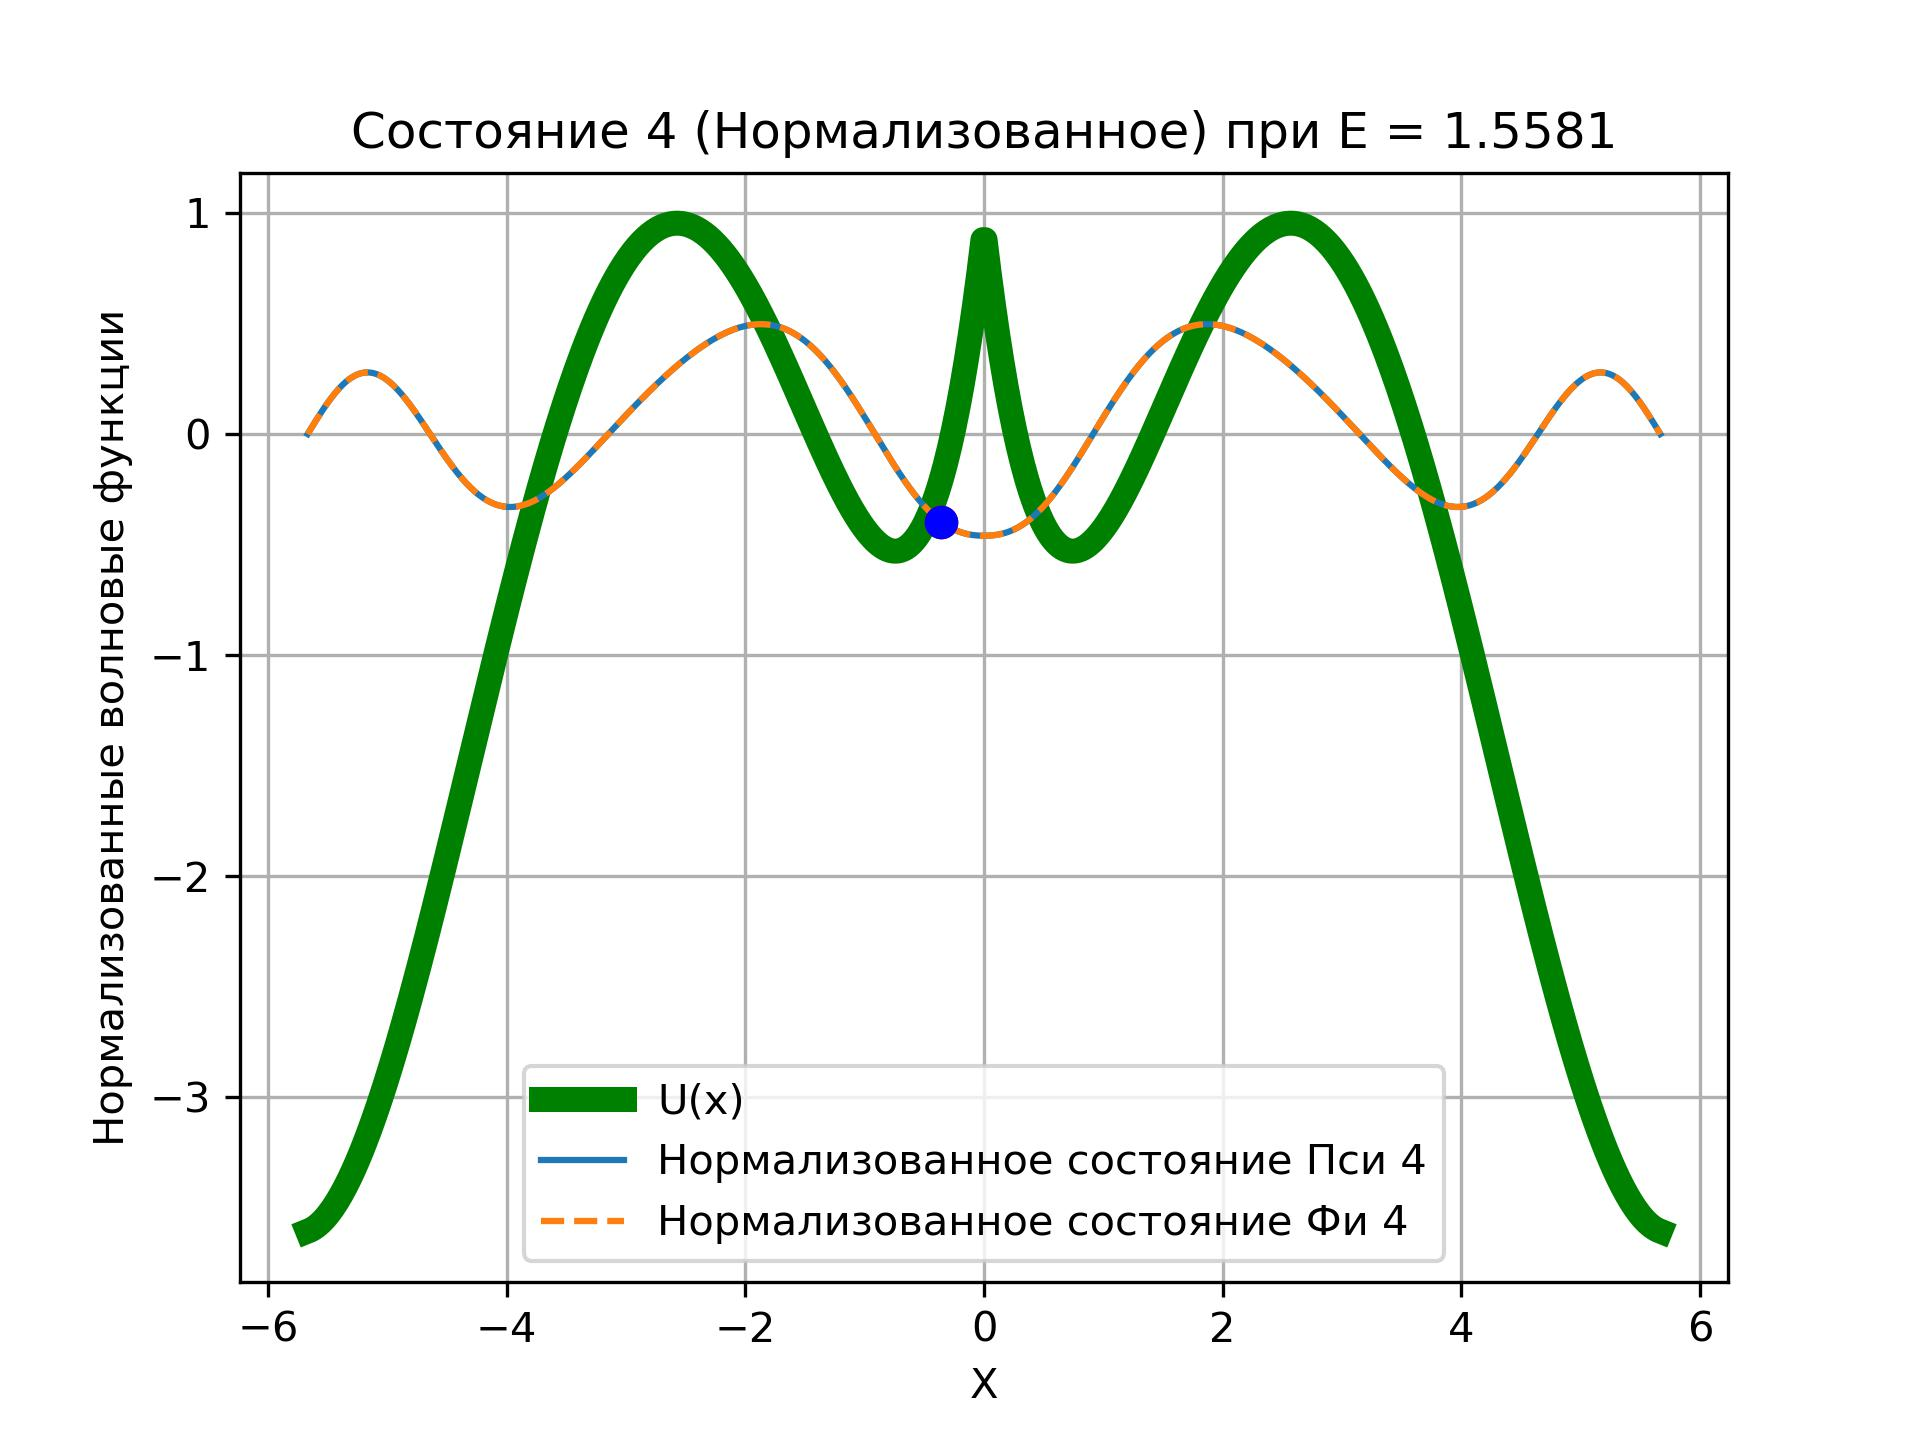
\includegraphics[width=0.44\textwidth]{Состояние 4 (нормализованное).jpg}} &
        \adjustbox{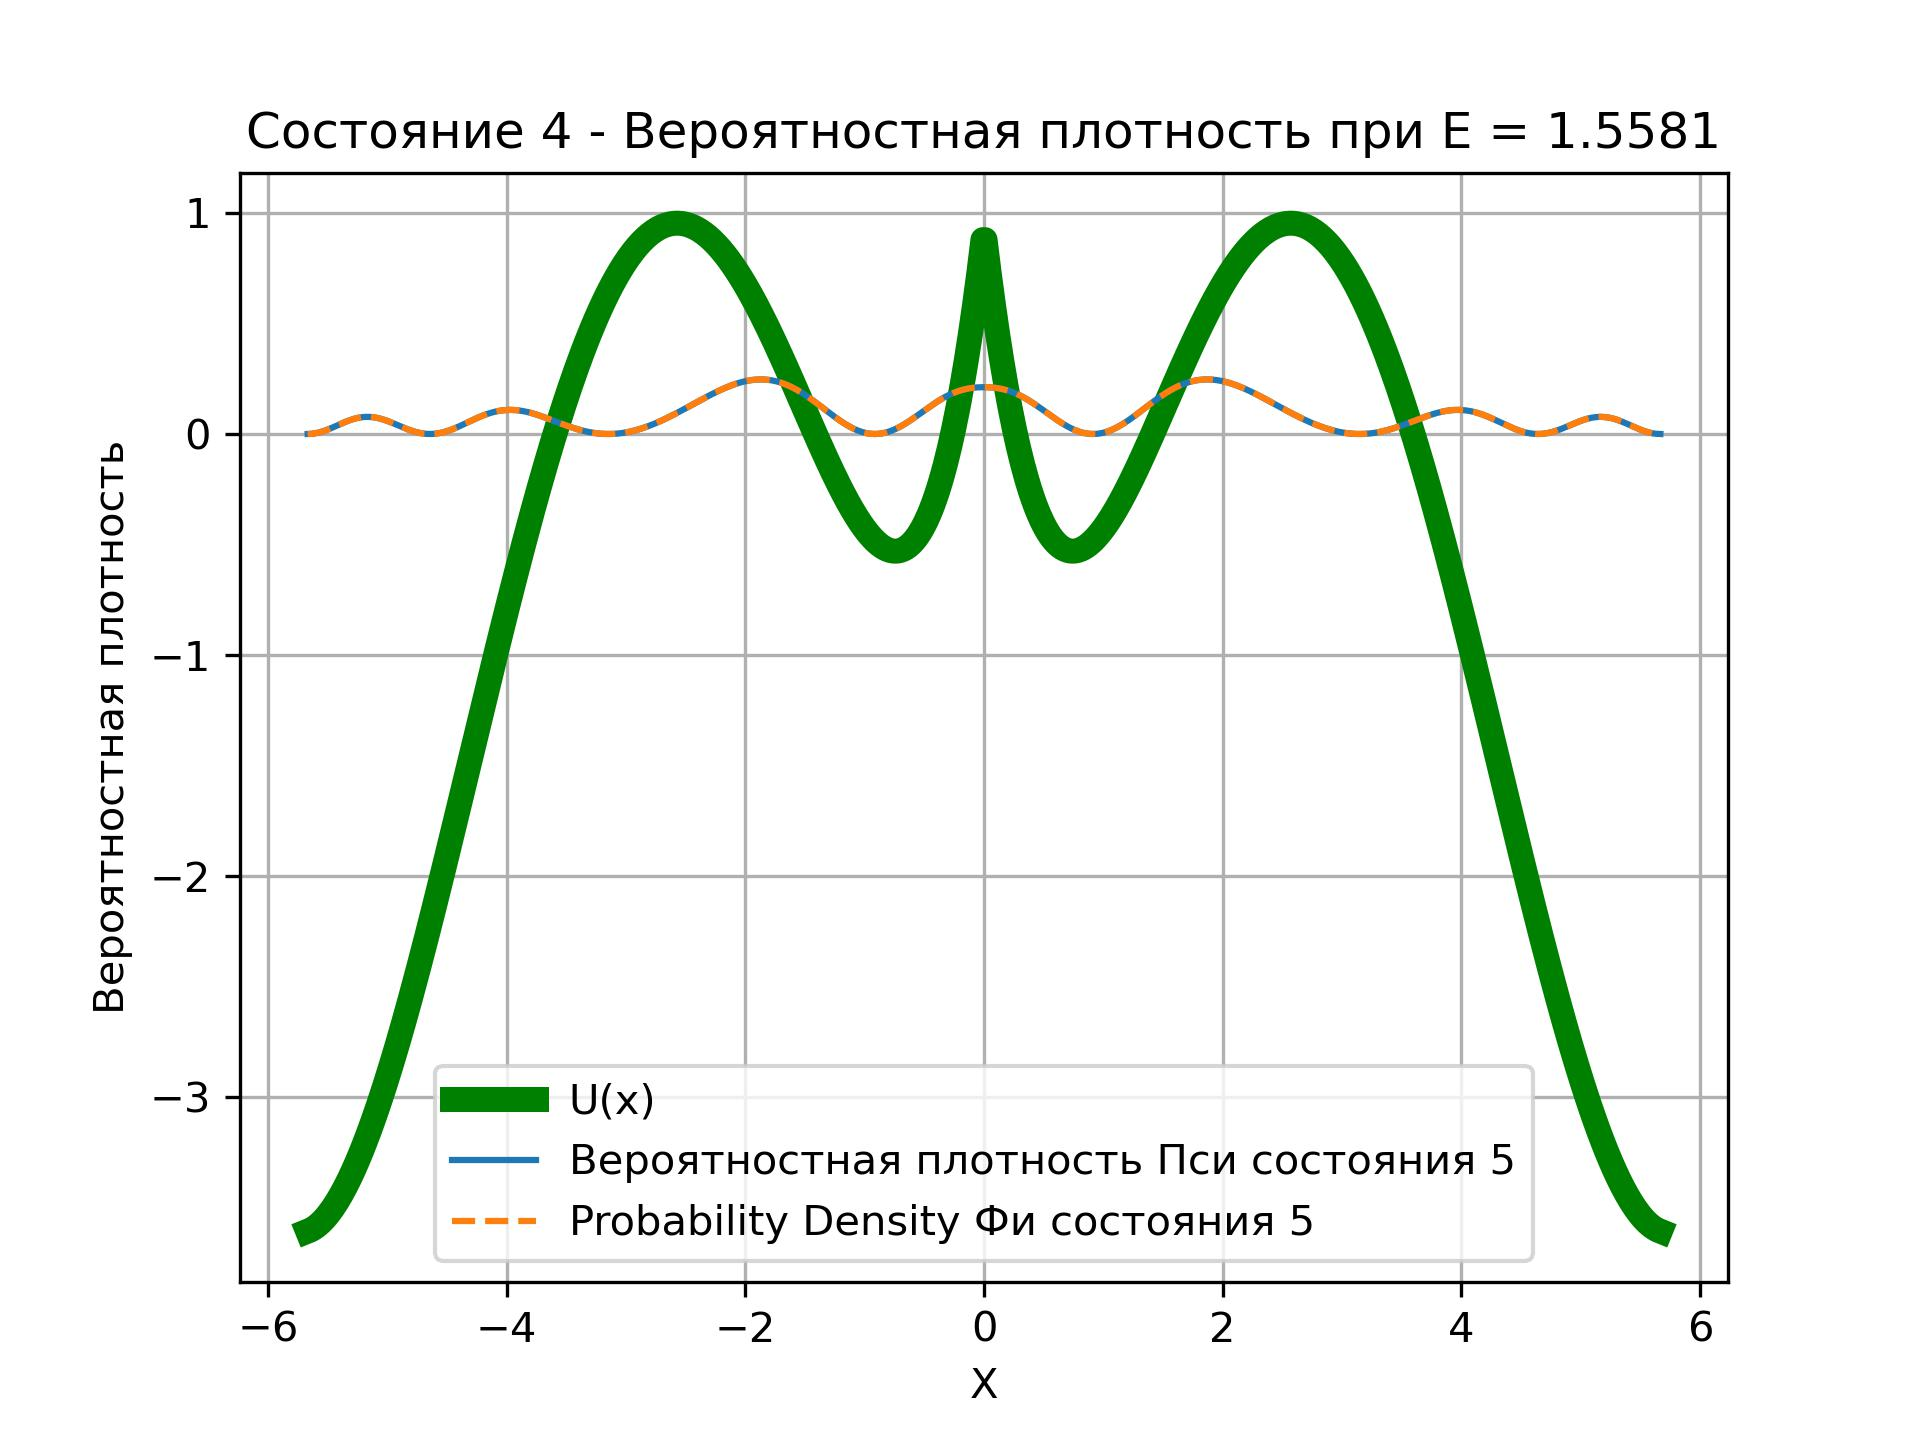
\includegraphics[width=0.44\textwidth]{Состояние 4 (Вероятностная плотность).jpg}} \\
        (a) Нормализованное состояние & (b) Вероятностная плотность
    \end{tabular}
    \caption{Графики для состояния 4}
    \label{fig:state_4}
\end{figure}

\begin{figure}[H]
    \centering
    \begin{tabular}{cc}
        \adjustbox{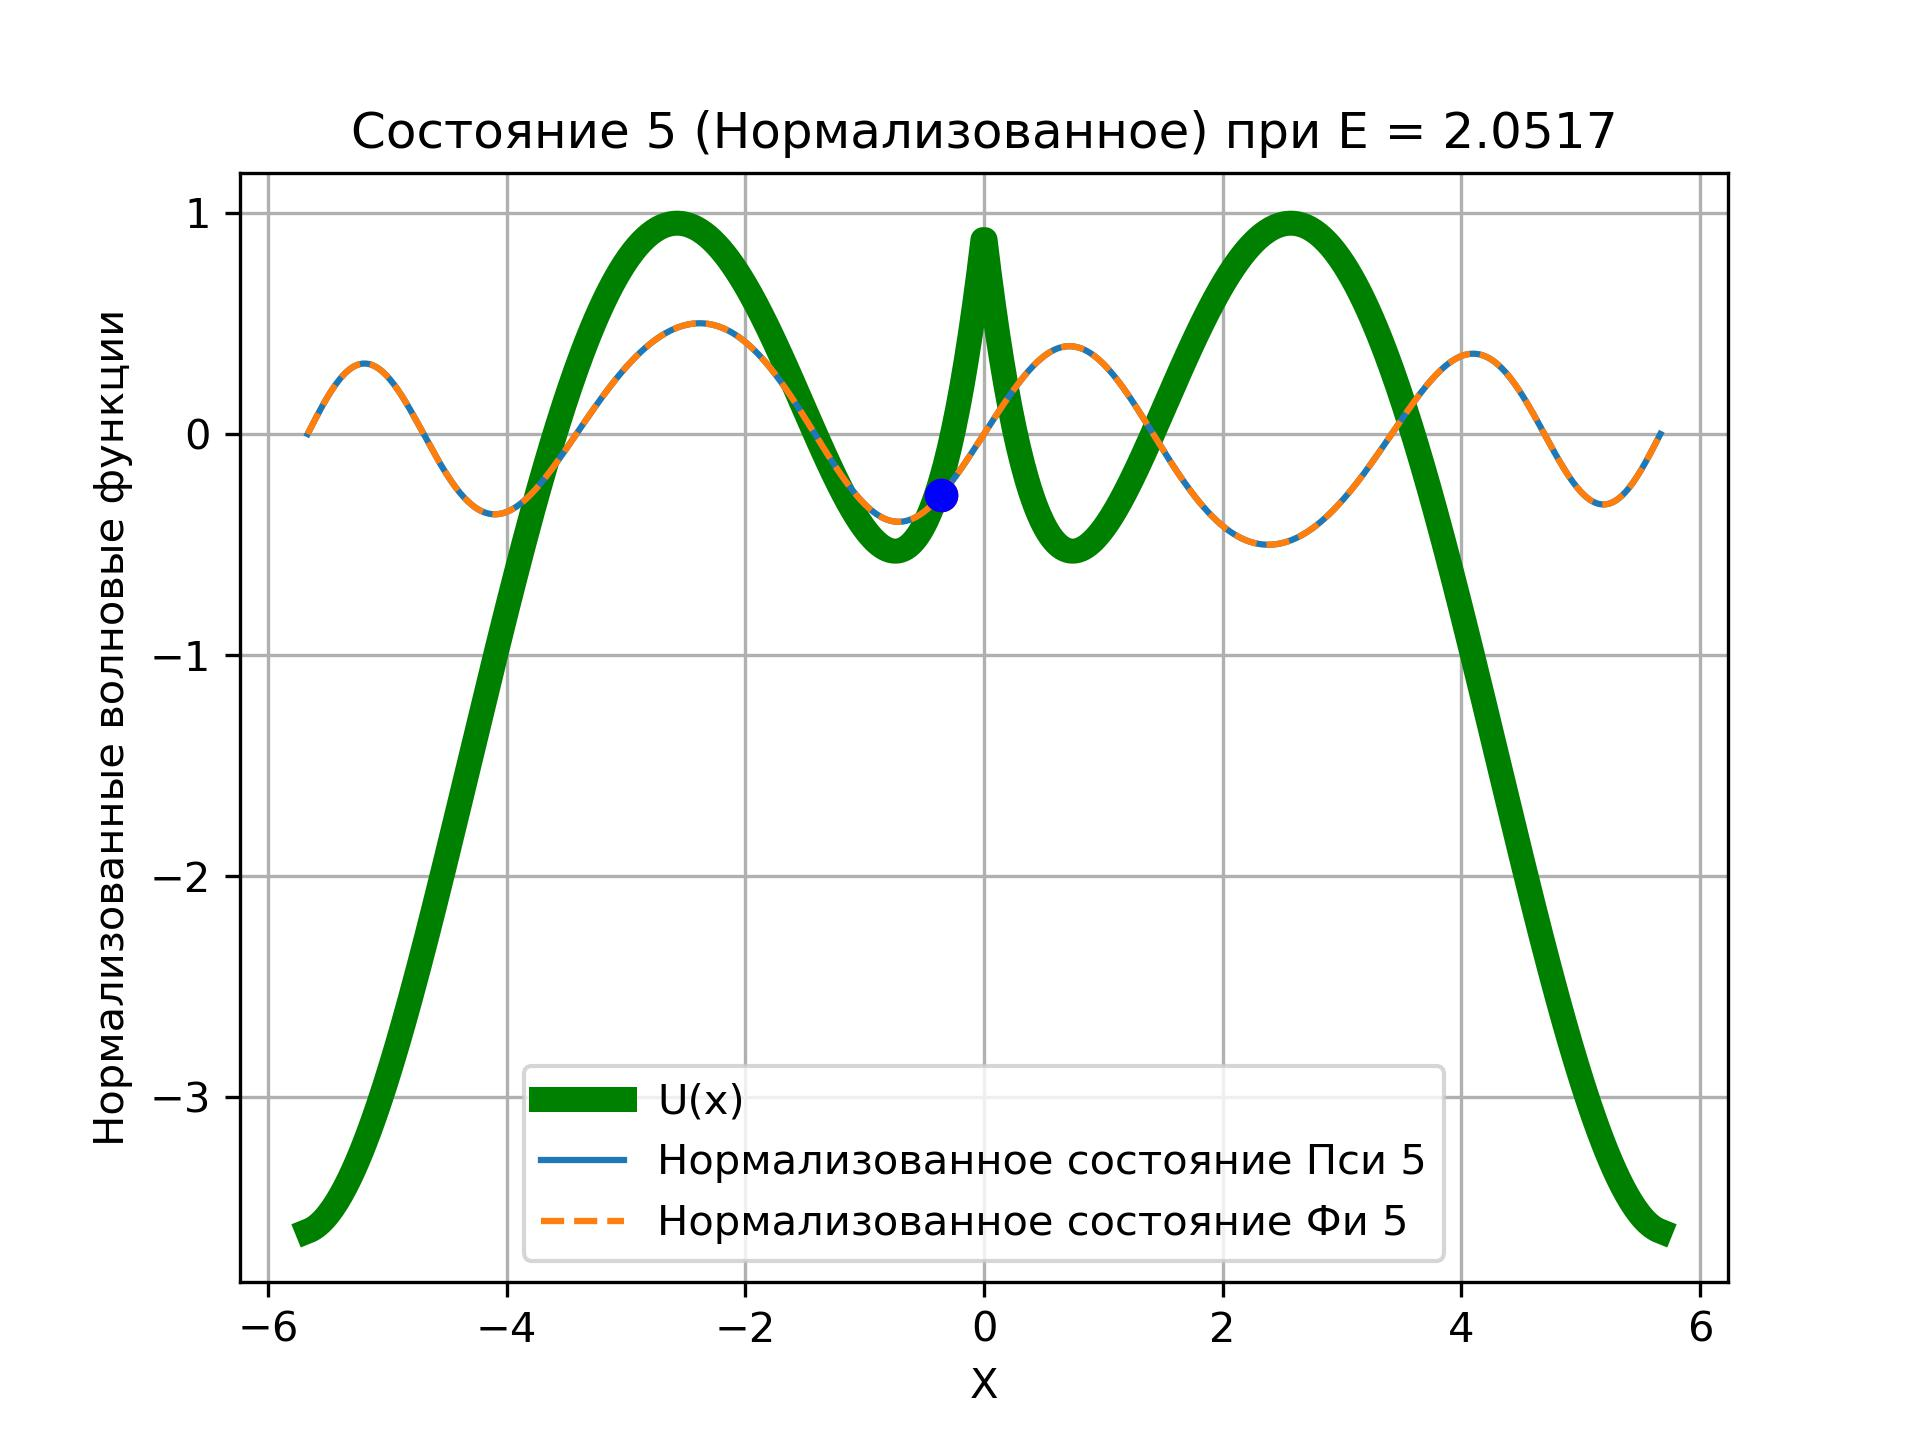
\includegraphics[width=0.44\textwidth]{Состояние 5 (нормализованное).jpg}} &
        \adjustbox{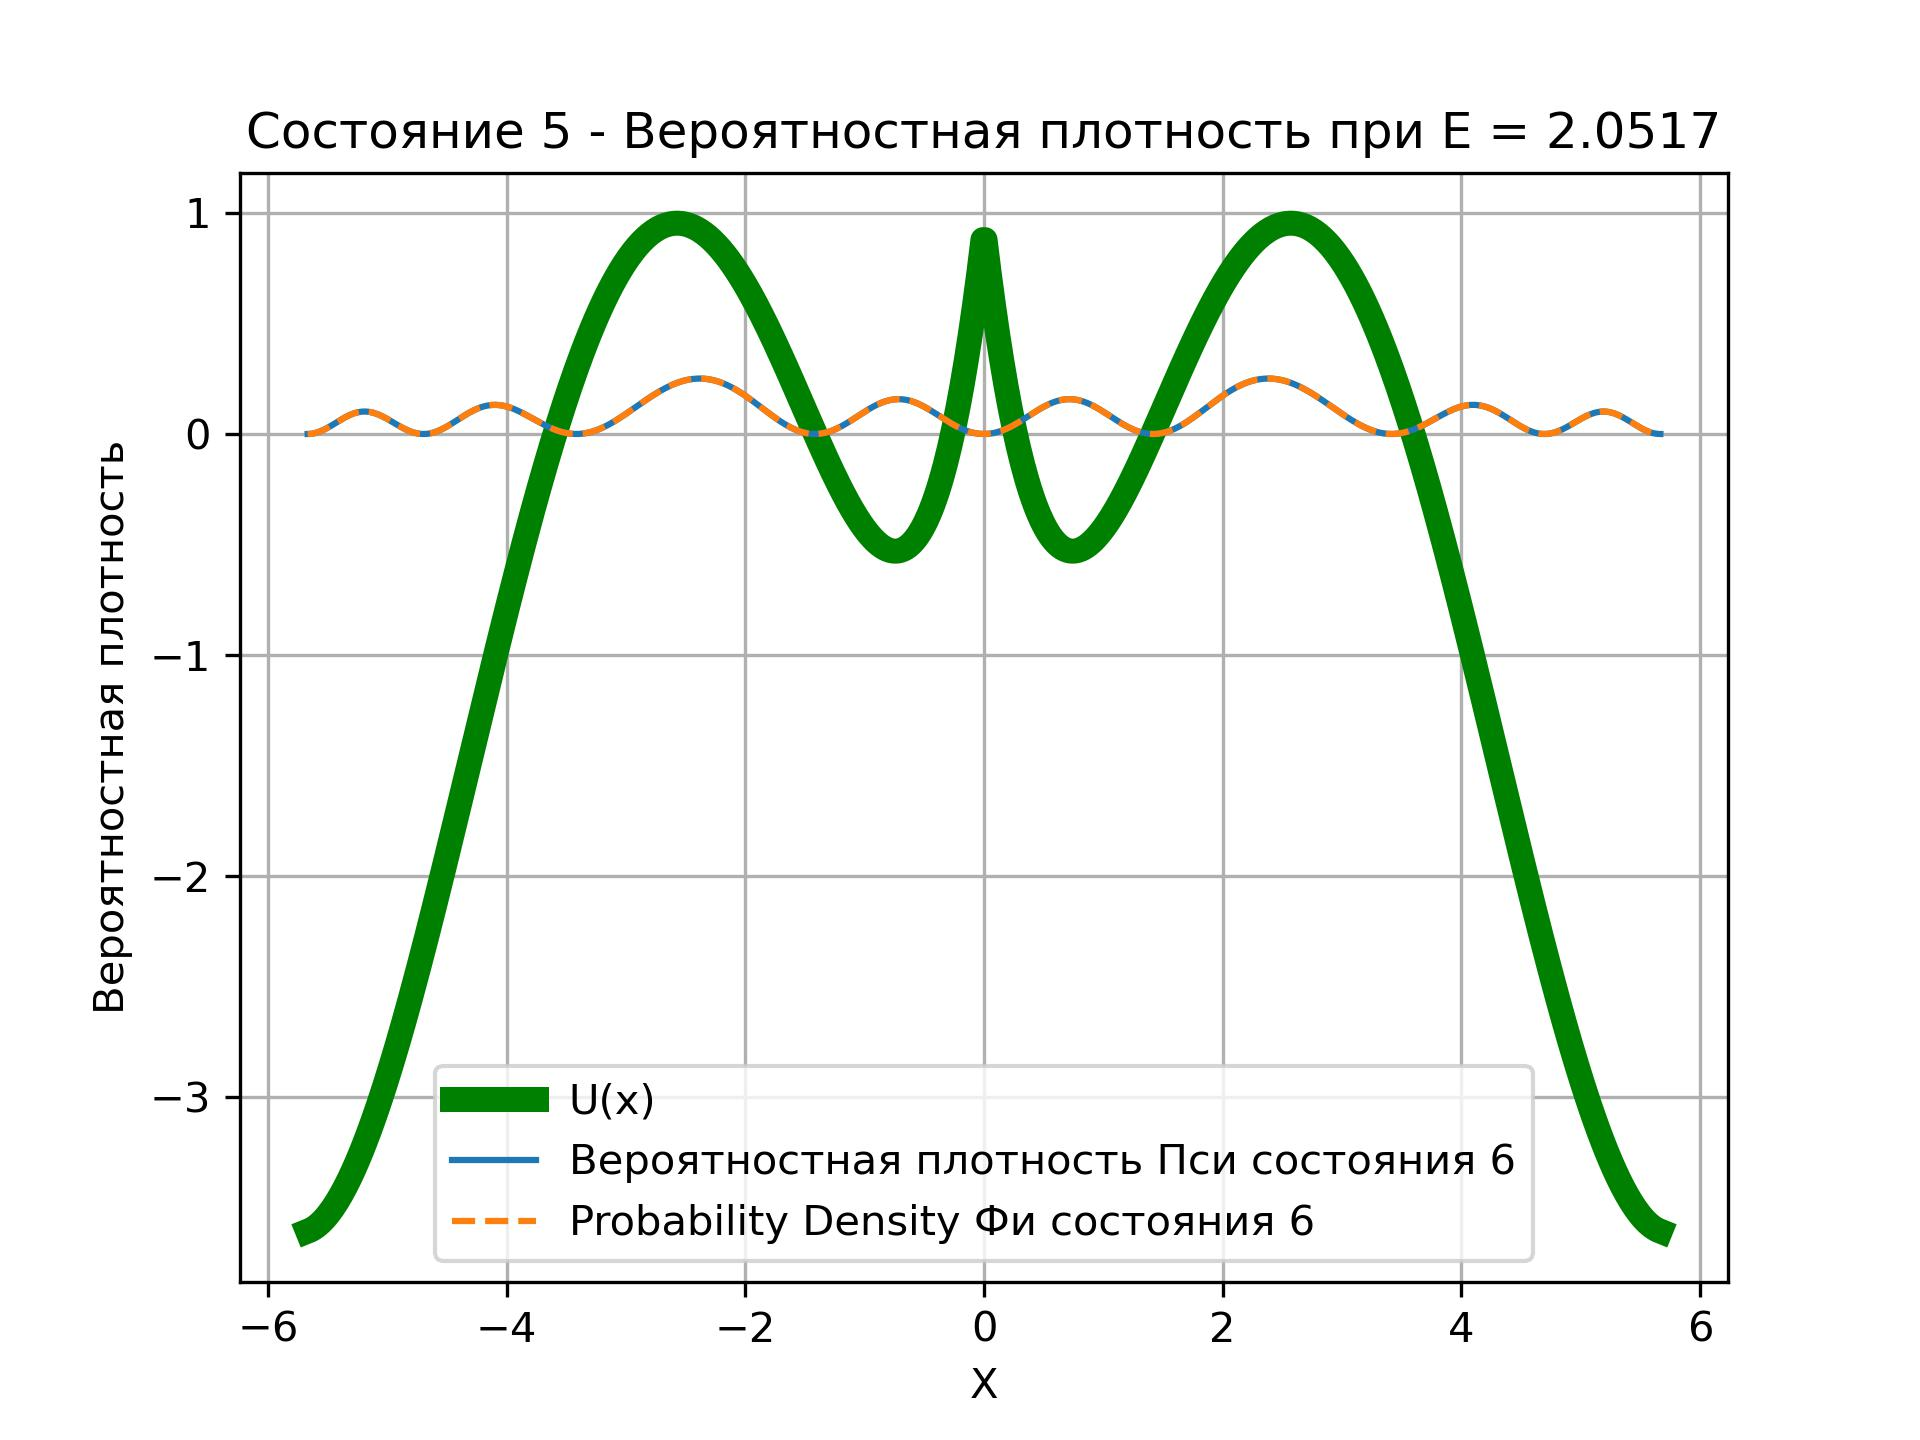
\includegraphics[width=0.44\textwidth]{Состояние 5 (Вероятностная плотность).jpg}} \\
        (a) Нормализованное состояние & (b) Вероятностная плотность
    \end{tabular}
    \caption{Графики для состояния 5}
    \label{fig:state_5}
\end{figure}

\begin{figure}[H]
    \centering
    \begin{tabular}{cc}
        \adjustbox{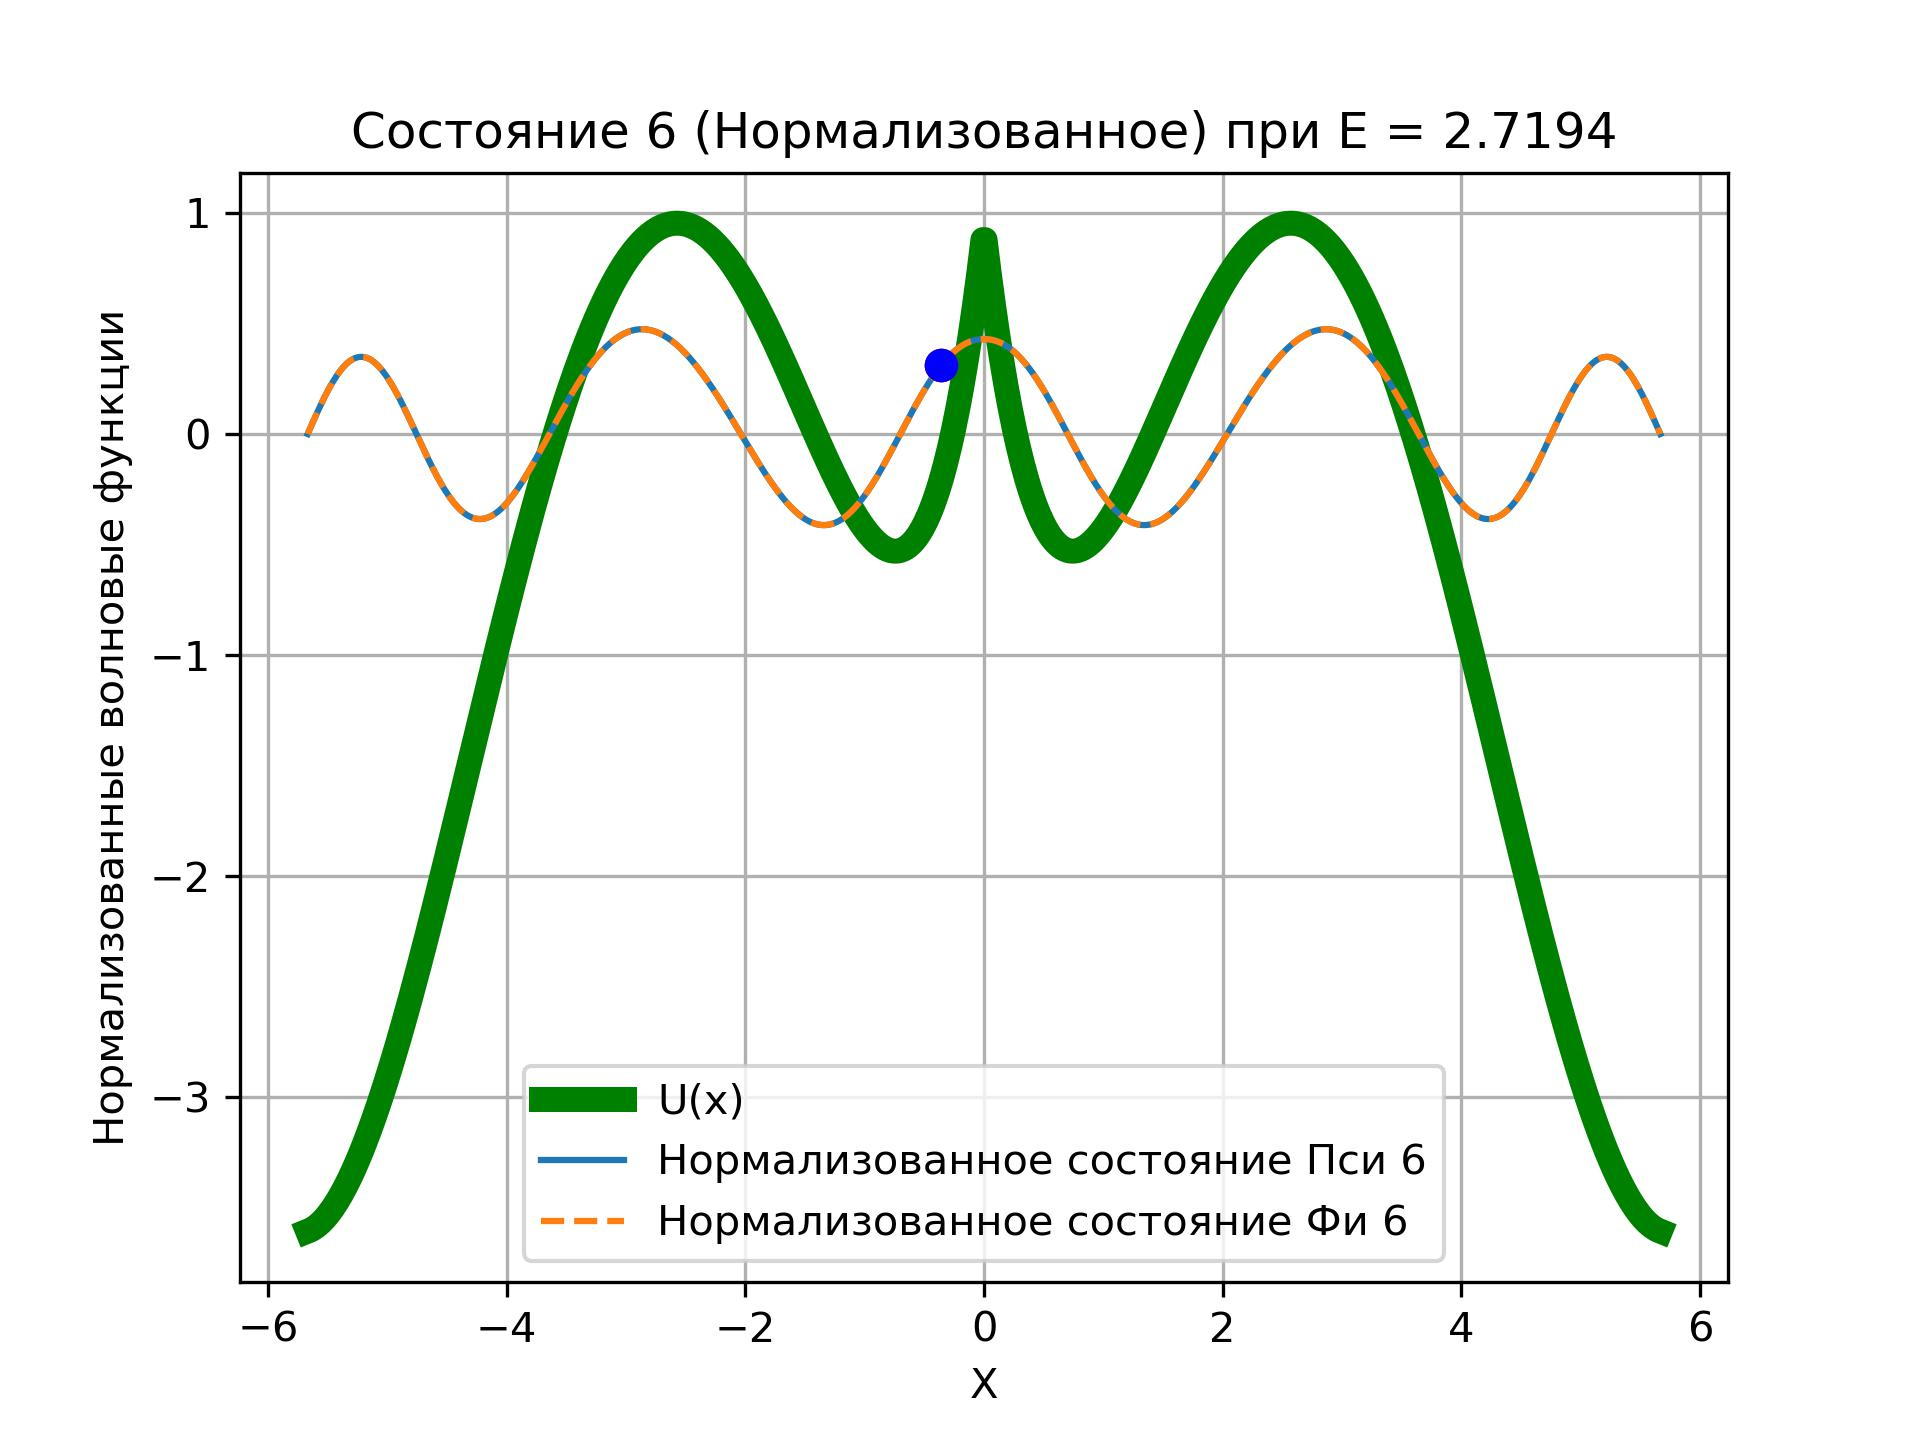
\includegraphics[width=0.44\textwidth]{Состояние 6 (нормализованное).jpg}} &
        \adjustbox{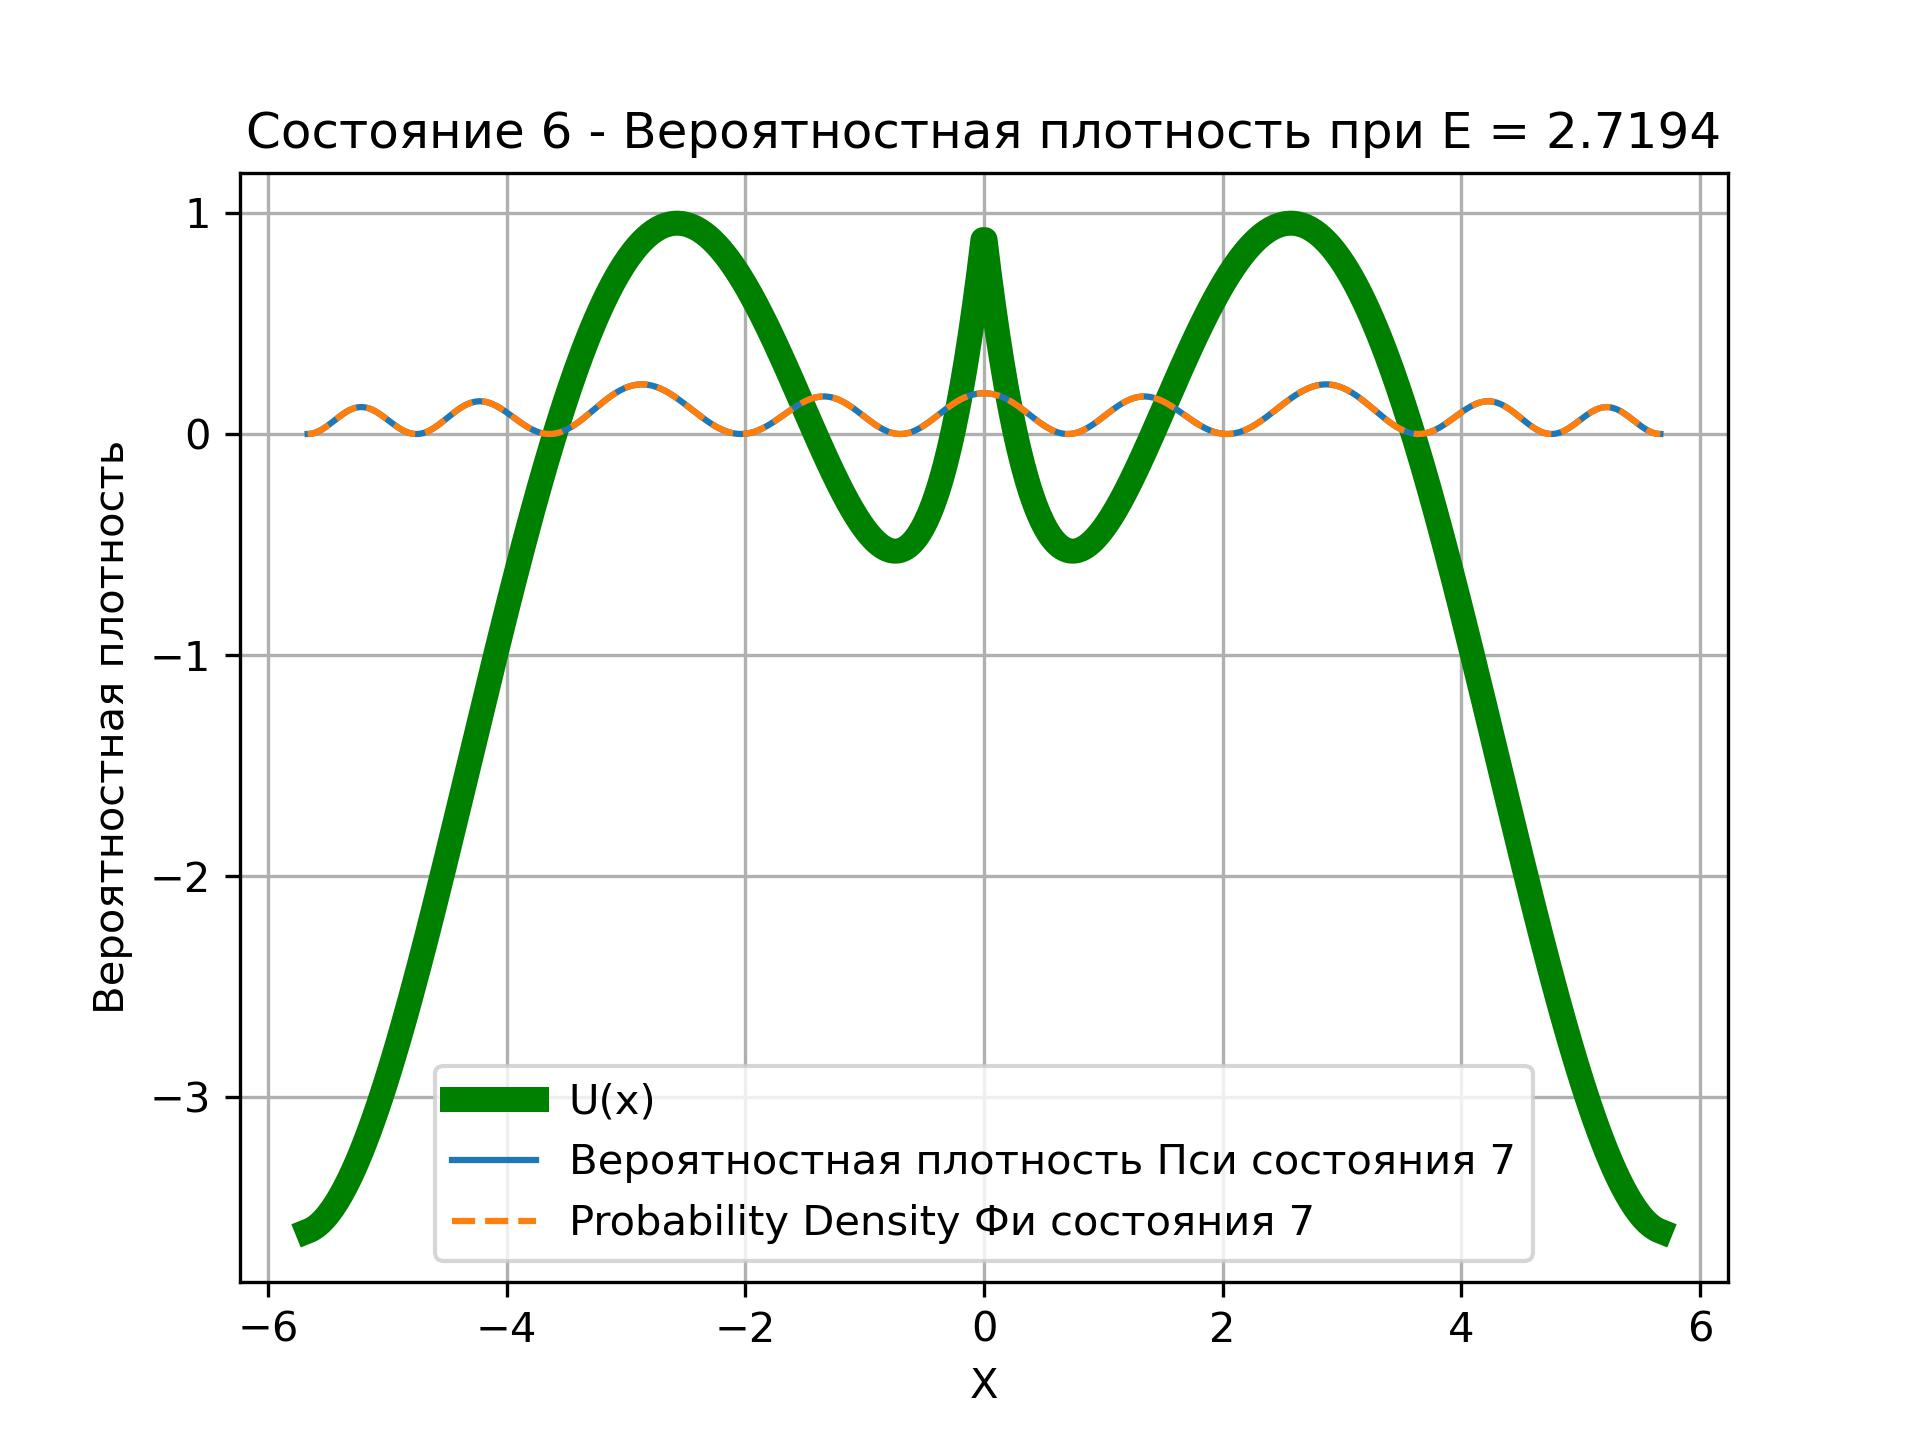
\includegraphics[width=0.44\textwidth]{Состояние 6 (Вероятностная плотность).jpg}} \\
        (a) Нормализованное состояние & (b) Вероятностная плотность
    \end{tabular}
    \caption{Графики для состояния 6}
    \label{fig:state_6}
\end{figure}

\newpage
\appendix
\section*{Приложение 1. Компьютерный код}
\begin{verbatim}
# Здесь может быть ваш Python-код решения уравнения Шрёдингера
# ...
\end{verbatim}

\newpage
\begin{thebibliography}{9}
\bibitem{landau} Ландау Л.Д., Лифшиц Е.М. \textit{Квантовая механика.} М.: Физматлит, 2004.
\bibitem{tim} Тимошенко Ю.К. \textit{Численное решение стационарного уравнения Шрёдингера.} Воронеж, 2019.
\bibitem{python} Бизли Д. \textit{Python. Подробный справочник.} СПб.: Символ-Плюс, 2010.
\end{thebibliography}

\end{document}
